\subsection{同态 F 与移位 V}

设 A 为一个环。在本段其余部分中，我们分别用 + 和 × 表示 W(A) 中的加法和乘法运算。我们还将 0 记作 0 \(_{A}\)，将 1 记作 \(1_{A}\)。我们按下列公式定义从 W(A) 到自身的两个映射 \(^{1}\) \(F_{A}\) 和 \(V_{A}\)（也简记为 F 和 V）。

\begin{enumerate}
\def\labelenumi{(\arabic{enumi})}
\setcounter{enumi}{22}
\tightlist
\item
\end{enumerate}

\[
\mathrm{F} _ {\mathbf {A}} (\boldsymbol {a}) = \big (\mathrm{F} _ {n} (a _ {0},..., a _ {n + 1}) \big) _ {n \in \mathbb {N}},\tag{24}
\]

\[
\mathrm{V} _ {\mathrm{A}} (\boldsymbol {a}) = (0, a _ {0}, a _ {1}, \dots)
\]

\((\text{其中 } \boldsymbol{a} = (a_n)_{n \in \mathbb{N}} \text{ 属于 } \mathrm{W(A)})\)。映射 \(V_A\) 称为移位。公式

\[
\Phi_ {n} \left(\mathrm{F} _ {0} (\boldsymbol {a}), \dots , \mathrm{F} _ {n} (\boldsymbol {a})\right) = \Phi_ {n + 1} \left(a _ {0}, \dots , a _ {n + 1}\right) \quad (n \in \mathbf {N})\tag{25}
\]

由 (15) 立即得到。它也可写成如下形式：

\[
\Phi_ {\mathrm{A}} \circ \mathrm{F} _ {\mathrm{A}} = f _ {\mathrm{A}} \circ \Phi_ {\mathrm{A}}.\tag{26}
\]

公式

\[
\Phi_ {\mathrm{A}} \circ \mathrm{V} _ {\mathrm{A}} = v _ {\mathrm{A}} \circ \Phi_ {\mathrm{A}}\tag{27}
\]

由关系 (3) 得到。

设 \(\rho : \mathbf{B} \to \mathbf{A}\) 为一个环同态。关系式

\begin{enumerate}
\def\labelenumi{(\arabic{enumi})}
\setcounter{enumi}{27}
\tightlist
\item
\end{enumerate}

\[
\mathbf {W} (\rho) \circ \mathrm{F} _ {\mathbf {B}} = \mathrm{F} _ {\mathbf {A}} \circ \mathbf {W} (\rho)\tag{29}
\]

\[
\mathrm{W} (\rho) \circ \mathrm{V} _ {\mathrm{B}} = \mathrm{V} _ {\mathrm{A}} \circ \mathrm{W} (\rho)
\]

由定义立即得到。

命题 3．——设 A 为一个环。

\begin{enumerate}
\def\labelenumi{\alph{enumi})}
\item
  映射 \(F_{A}\) 是环 W(A) 的自同态。
\item
  映射 \(V_{A}\) 是环 \(\mathbf{W}(\mathbf{A})\) 的底层加法群的自同态。
\item
  对 W(A) 中的每个 a，都有 \(F_{A}(V_{A}(a)) = p.a\)（即 W(A) 中 p 个等于 a 的项之和）。
\item
  对 W(A) 中的任意 \(a\) 和 \(b\)，都有
\end{enumerate}

\begin{enumerate}
\def\labelenumi{(\arabic{enumi})}
\setcounter{enumi}{29}
\tightlist
\item
\end{enumerate}

\[
\mathrm{V} _ {\mathrm{A}} (a \times \mathrm{F} _ {\mathrm{A}} (b)) = \mathrm{V} _ {\mathrm{A}} (a) \times b\tag{31}
\]

\[
\mathrm{V} _ {\mathrm{A}} (a) \times \mathrm{V} _ {\mathrm{A}} (b) = p. \mathrm{V} _ {\mathrm{A}} (a \times b)
\]

（即 W(A) 中 p 个等于 \(V_A(a \times b)\) 的项之和）。

\begin{enumerate}
\def\labelenumi{\alph{enumi})}
\setcounter{enumi}{4}
\tightlist
\item
  置 \(\mu = V_{A}(1) = (0, 1, 0, \ldots)\)。对 W(A) 中的每个 \(b\)，都有
\end{enumerate}

\[
\mathrm{V} _ {\mathrm{A}} \left(\mathrm{F} _ {\mathrm{A}} (\boldsymbol {b})\right) = \mu \times \boldsymbol {b}.\tag{32}
\]

\begin{enumerate}
\def\labelenumi{\alph{enumi})}
\setcounter{enumi}{5}
\tightlist
\item
  对 W(A) 的每个元素 \(\mathbf{a}\)，记 W(A) 中 p 个等于 a 的元素的乘积为 \(\mathbf{a}^{*p}\)。则有
\end{enumerate}

\[
\mathrm{F} _ {\mathbf {A}} (\boldsymbol {a}) \equiv \boldsymbol {a} ^ {* p} \bmod p. \mathrm{W} (\mathbf {A}) \quad (\text { ideal of } \mathrm{W} (\mathbf {A}) \text { generated by } p. \mathbf {1}).\tag{33}
\]

设 \(\rho: \mathbf{B} \to \mathbf{A}\) 为满足第 4 节引理 3 条件的环同态。于是 \(\mathbf{W}(\rho): \mathbf{W}(\mathbf{B}) \to \mathbf{W}(\mathbf{A})\) 是满射环同态，而 \(\Phi_{\mathbf{B}}: \mathbf{W}(\mathbf{B}) \to \mathbf{B}^{\mathbf{N}}\) 是单射环同态。此外，\(f_{\mathbf{B}}: \mathbf{B}^{\mathbf{N}} \to \mathbf{B}^{\mathbf{N}}\) 是环同态。由公式 (26) 和 (28)，有

\[
\Phi_ {\mathrm{B}} \circ \mathrm{F} _ {\mathrm{B}} = f _ {\mathrm{B}} \circ \Phi_ {\mathrm{B}}, \quad \mathrm{W} (\rho) \circ \mathrm{F} _ {\mathrm{B}} = \mathrm{F} _ {\mathrm{A}} \circ \mathrm{W} (\rho),
\]

因此断言 a) 立即成立。断言 b) 同理，由公式 (27)、(29) 以及 \(v_{B}\) 是 \(B^{N}\) 的底层加法群的自同态这一事实得到。

设 \(\pmb{a}\) 是 W(A) 的一个元素，并取 W(B) 中的元素 \(\pmb{x}\)，使其在 W(ρ) 下的像为 \(\pmb{a}\)。置 \(\xi = \Phi_{\mathrm{B}}(\pmb{x})\)。由 \(f_{\mathrm{B}}\) 和 \(v_{\mathrm{B}}\) 的定义立即得到 \(f_{\mathrm{B}}(v_{\mathrm{B}}(\xi)) = p.\xi\)（即 B \(^{\mathbf{N}}\) 中 \(p\) 个等于 \(\xi\) 的项之和）。根据公式 (26)、(27)（其中以 B 代替 A），W(B) 中的元素 F \(_{\mathrm{B}}\) (V \(_{\mathrm{B}}\) ( \(\pmb{x}\) )) 和 \(p.\pmb{x}\) 具有相同的像 \(p.\xi\)（经由单射 \(\Phi_{\mathrm{B}}\)），因而相等。于是，公式 F \(_{\mathrm{A}}\) (V \(_{\mathrm{A}}\) ( \(\pmb{a}\) )) = \(p.\pmb{a}\) 由关系 (28)、(29) 得到。这就证明了 \(c\)。

同理，公式 (30) 的证明归结为证明关系式

\[
v _ {\mathrm{B}} (\xi f _ {\mathrm{B}} (\eta)) = v _ {\mathrm{B}} (\xi) \eta
\]

其中 \(\xi\)、\(\eta\) 属于 B \(^{N}\)。这由等式

\[
\begin{array}{l} \xi f _ {\mathrm{B}} (\eta) = (\xi_ {0} \eta_ {1}, \xi_ {1} \eta_ {2}, \dots) \\ v _ {\mathrm{B}} (\xi) \eta = (0, p \xi_ {0} \eta_ {1}, p \xi_ {1} \eta_ {2}, \dots). \end{array}
\]

考虑到 (b)、(c)，公式 (31) 由公式 (30) 得到，其中 \(\boldsymbol{b}\) 被 \(\mathrm{V}_{\mathbf{A}}(\boldsymbol{b})\) 所代替。公式 (32) 是公式 (30) 在 \(\boldsymbol{a} = \boldsymbol{1}\) 时的特例。

类似地，公式 (33) 的证明归结为证明关系式

\[
f _ {\mathrm{B}} (\xi) \equiv \xi^ {p} \bmod p. \Phi_ {\mathrm{B}} (\mathrm{B} ^ {\mathbf {N}}),
\]

其中 \(\xi^{p}\) 表示 \(\mathbf{B}^{\mathbf{N}}\) 中 \(p\) 个等于 \(\xi\) 的元素的乘积。根据第 2 节命题 2 的 c)，这等价于：对每个 \(n \geqslant 0\)，都有

\[
\sigma \left(\xi_ {n + 1} - \xi_ {n} ^ {p}\right) \equiv \xi_ {n + 2} - \xi_ {n + 1} ^ {p} \bmod p ^ {n + 2} \mathbf {B}.
\]

现在，对每个 \(n \geqslant 0\)，由上引文有

\[
\sigma (\xi_ {n}) \equiv \xi_ {n + 1} \bmod p ^ {n + 1} \mathbf {B}
\]

因为 \(\xi = \Phi_{\mathbf{B}}(\boldsymbol{x})\)；由此借助第 1 节引理 1 可推出

\[
\sigma (\xi_ {n}) ^ {p} \equiv \xi_ {n + 1} ^ {p} \bmod p ^ {n + 2} \mathbf {B}.
\]

这就证明了所需的关系式。

注记．——关于在普适 Witt 环情形下与映射 F、V 类似的映射的定义，见第 52 页及以下的习题 36、37、38。

\subsection{环 W(A) 的滤子与拓扑}

引理 4．——设 A 为一个环，\(m \geqslant 1\) 为整数。则有

\[
\boldsymbol {a} = \left(a _ {0}, \dots , a _ {m - 1}, 0, \dots\right) + \underbrace {\left(0 , \dots , 0 , \right.} _ {m \text { terms }}, a _ {m}, a _ {m + 1}, \dots)\tag{34}
\]

对 W(A) 中的所有 a 均成立。

设 \(\rho: B \to A\) 为一个满足第 4 节引理 3 条件的环同态。于是 \(W(\rho): W(B) \to W(A)\) 是一个满射环同态，而 \(\Phi_B: W(B) \to B^N\) 是一个单射同态。因此，只需证明有

\[
\Phi_ {n} (\boldsymbol {b}) = \Phi_ {n} (b _ {0},..., b _ {m - 1}, 0,...) + \Phi_ {n} (0,..., 0, b _ {m}, b _ {m + 1},...) \tag{35}
\]

对于 W(B) 中的所有 b 以及所有整数 \(m \geqslant 1, n \geqslant 0\)，均成立。现在有

\[
\begin{array}{r l} \Phi_ {n} (b _ {0},..., b _ {m - 1},... \dots) & = \Phi_ {n} (b _ {0},..., b _ {n}) \quad \text { if } \quad 0 \leqslant n <   m \\ & = \sum_ {i = 0} ^ {m - 1} p ^ {i}. b _ {i} ^ {p ^ {n - i}} \quad \text { if } \quad m \leqslant n \end{array}
\]

\[
\begin{array}{r l} \Phi_ {n} (0, \dots , 0, b _ {m}, b _ {m + 1}, \dots) & = 0 \\ & = \sum_ {i = m} ^ {n} p ^ {i}. b _ {i} ^ {p ^ {n - i}} \end{array} \quad \text { if } \quad 0 \leqslant n <   m \quad \text { if } \quad m \leqslant n,
\]

从而得到公式 (35)。

设 A 为一个环。对于每个整数 \(m \geqslant 0\)，记 \(\mathbf{V}_{m}(\mathbf{A})\) 为 Witt 向量 \(\boldsymbol{a} = (a_{n})_{n \in \mathbb{N}}\) 所成的集合，其中 \(a_{n} = 0\) 对 \(0 \leqslant n < m\) 成立。它是 \(m\) 次幂 \(\mathbf{V}^{m}\)（由映射 \(\mathbf{V}_{\mathrm{A}}\) 得到）的像。公式

\begin{enumerate}
\def\labelenumi{(\arabic{enumi})}
\setcounter{enumi}{35}
\tightlist
\item
\end{enumerate}

\[
\mathrm{V} ^ {m} (\boldsymbol {a} + \boldsymbol {b}) = \mathrm{V} ^ {m} (\boldsymbol {a}) + \mathrm{V} ^ {m} (\boldsymbol {b})\tag{37}
\]

\[
\mathrm{V} ^ {m} (a) \times b = \mathrm{V} ^ {m} (a \times \mathrm{F} ^ {m} (b))
\]

由第 5 节命题 3 对 m 归纳得到。它们蕴含 V \(_{m}\) (A) 是 W(A) 的理想。

\pandocbounded{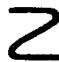
\includegraphics[keepaspectratio]{images/part001_18cee607.jpg}}

置 \(\mathrm{V}_{m}(\mathrm{A}) = \mathrm{W}(\mathrm{A})\)，当 \(m < 0\) 时。序列 \((\mathrm{V}_{m}(\mathrm{A}))_{m \in \mathbf{Z}}\) 是环 \(\mathrm{W}(\mathrm{A})\) 的加法群上的降滤子。它与 \(\mathrm{W}(\mathrm{A})\) 的环结构相容（III，第 2 节第 1 号定义 2）当且仅当 A 是特征为 \(p\) 的环（参见第 3 节例 2 及下文第 8 节命题 5 的推论）。

下文在 W(A) 上赋予拓扑 \(\mathcal{G}\)，它与滤子 \((\mathrm{V}_m(\mathrm{A}))_{m\in \mathbf{Z}}\) 关联。由于 \(\mathrm{V}_m(\mathrm{A})\) 对所有 \(m\in \mathbf{Z}\) 都是 W(A) 的理想，拓扑 \(\mathcal{G}\) 与 W(A) 的环结构相容（TG，III，第 49 页，例 3）。设 \(a\in \mathrm{W(A)}\)；集合 \(a + \mathrm{V}_m(\mathrm{A})\)，其中 \(m\) 遍历 N，构成 \(a\) 关于 \(\mathcal{G}\) 的邻域基。由引理 4 可知，\(a + \mathrm{V}_m(\mathrm{A})\) 由 Witt 向量 \(b\) 组成，并满足 \(a_i = b_i\)（\(0\leqslant i < m\)）。因此，\(\mathcal{G}\) 正是 \(\mathbf{A}^{\mathbf{N}}\) 上各因子离散拓扑的乘积拓扑，故 W(A) 是一个 Hausdorff 且完备的拓扑环（TG，II，第 17 页，命题 10，以及 TG，III，第 22 页，命题 4）。

记 \(\tau_{\mathbf{A}}\)（或简记为 \(\tau\)）为从 A 到 W(A) 的映射，它把 \((a, 0, 0, \ldots)\) 与 A 的每个元素 \(a\) 关联起来。我们有 \(\Phi_n(\tau(a)) = a^{p^n}\)，对每个 \(n \in \mathbb{N}\) 均成立。对任意环同态 \(\rho: \mathbf{B} \to \mathbf{A}\)，都有 W( \(\rho\) ) \(\circ\) \(\tau_{\mathbf{B}} = \tau_{\mathbf{A}} \circ \rho\)。

命题 4．——设 \(a\) 和 \(b\) 属于 \(\mathbf{A}\)，且 \(\boldsymbol{x} = (x_n)_{n \in \mathbb{N}}\) 是 \(\mathbf{W}(\mathbf{A})\) 的一个元素。

\begin{enumerate}
\def\labelenumi{\alph{enumi})}
\tightlist
\item
  有如下公式
\end{enumerate}

\begin{enumerate}
\def\labelenumi{(\arabic{enumi})}
\setcounter{enumi}{37}
\tightlist
\item
\end{enumerate}

\[
\tau (a b) = \tau (a) \times \tau (b)\tag{39}
\]

\[
\tau (a) \times x = (a ^ {p ^ {n}} x _ {n}) _ {n \in \mathbf {N}}.
\]

\begin{enumerate}
\def\labelenumi{\alph{enumi})}
\setcounter{enumi}{1}
\tightlist
\item
  通项为 \(\mathbf{V}^{n}(\tau(x_{n}))\) 的级数在 \(\mathbf{W}(\mathbf{A})\) 中收敛，且其和为 \(x\)。
\end{enumerate}

设 \(n\) 为正整数。第 3 节引入的多项式 \(\mathbf{P}_{n}(\mathbf{X}_{0},\ldots,\mathbf{X}_{n};\mathbf{Y}_{0},\ldots,\mathbf{Y}_{n})\) 是权为 \(p^{n}\) 的关于族 \((\mathbf{X}_{0},\ldots,\mathbf{X}_{n})\) 的等压多项式，其中赋予 \(\mathbf{X}_{i}\) 权 \(p^{i}\)。因此有

\[
\mathrm{P} _ {n} \left(\mathrm{X} _ {0}, 0, \dots , 0; \mathrm{Y} _ {0}, \dots , \mathrm{Y} _ {n}\right) = \mathrm{X} _ {0} ^ {p ^ {n}} \mathrm{P} _ {n} (1, 0, \dots , 0; \mathrm{Y} _ {0}, \dots , \mathrm{Y} _ {n}).\tag{40}
\]

由于 1 = (1, 0, 0, \ldots) 是系数环为 \(\mathbf{Z}[(X_n)_{n\in\mathbb{N}}, (Y_n)_{n\in\mathbb{N}}]\) 的 Witt 向量环的单位元，所以有

\[
\mathrm{P} _ {n} (1, 0,..., 0; \mathrm{Y} _ {0},..., \mathrm{Y} _ {n}) = \mathrm{Y} _ {n}.\tag{41}
\]

以 \(a\) 代替 \(\mathbf{X}_{0}\)，以 \(x_{i}\) 代替 \(\mathbf{Y}_{i}\)，由 (40)、(41) 得到关系式：

\[
\mathrm{P} _ {n} (a, 0, \dots , 0; x _ {0}, \dots , x _ {n}) = a ^ {p ^ {n}} x _ {n}.
\]

根据 W(A) 中乘法的定义，(39) 得证；公式 (38) 是 (39) 的特例。

证明 \(b\)。按定义，\(\mathbf{V}^{n}(\tau(x_{n}))\) 是一个所有分量均为零、但下标为 \(n\) 的分量等于 \(x_{n}\) 的序列。由引理 4 对 \(m\) 归纳可得

\[
\sum_ {n = 0} ^ {m} \mathrm{V} ^ {n} (\tau (x _ {n})) = (x _ {0},..., x _ {m}, 0, 0,...)
\]

对每个整数 \(m \geqslant 0\) 均成立；取极限即得 \(b\)，因为 W(A) 上的拓扑 \(\mathcal{C}\) 是各因子 A 的离散拓扑的乘积。

\subsection{\texorpdfstring{\(W_{n}(A)\) 的有限长度 Witt 向量环}{W\_\{n\}(A) 的有限长度 Witt 向量环}}

定义 2．——设 A 为一个环，\(n \geqslant 1\) 为整数。记 \(\mathbf{W}_{n}(\mathbf{A})\) 为商环 \(\mathbf{W}(\mathbf{A}) / \mathbf{V}_{n}(\mathbf{A})\)。

给定 A 中的元素 \(a_0, \ldots, a_{n-1}\)，将类 \([a_0, \ldots, a_{n-1}]\) 或 \([a_i]_{0 \leq i < n}\) 记作 \(\mathrm{V}_n(\mathrm{A})\) 模元素 \((a_0, \ldots, a_{n-1}, 0, 0, \ldots)\)（属于 \(\mathrm{W}(\mathrm{A})\)）的类。根据第 6 节引理 4，映射 \((a_0, \ldots, a_{n-1}) \mapsto [a_0, \ldots, a_{n-1}]\)（从 \(\mathrm{A}^n\) 到 \(\mathrm{W}_n(\mathrm{A})\)）是双射。因此，称 \(\mathrm{W}_n(\mathrm{A})\) 的元素为长度为 \(n\) 的 Witt 向量；类比地，\(\mathrm{W}(\mathrm{A})\) 的元素

有时也称为无限长度的 Witt 向量。记 \(\pi_n\) 为从 W(A) 到 \(\mathrm{W}_n(\mathrm{A})\) 的典范同态。根据第 6 节引理 4，有

\[
\pi_ {n} (\boldsymbol {a}) = [ a _ {0}, \dots , a _ {n - 1} ]\tag{42}
\]

对 W(A) 中的每个 \(\boldsymbol{a} = (a_{n})_{n \in \mathbb{N}}\) 均成立。

根据 W(A) 中运算的定义，\(\mathrm{W}_{n}(\mathrm{A})\) 中的运算可如下描述：

\[
\begin{array}{r l} & {[ a _ {0},..., a _ {n - 1} ] + [ b _ {0},..., b _ {n - 1} ] = [ \mathrm{S} _ {i} (a _ {0},..., a _ {i}; b _ {0},..., b _ {i}) ] _ {0 \leqslant i <   n}} \\ & {[ a _ {0},..., a _ {n - 1} ] \times [ b _ {0},..., b _ {n - 1} ] = [ \mathrm{P} _ {i} (a _ {0},..., a _ {i}; b _ {0},..., b _ {i}) ] _ {0 \leqslant i <   n}} \\ & {\quad - [ a _ {0},..., a _ {n - 1} ] = [ \mathrm{I} _ {i} (a _ {0},..., a _ {i}) ] _ {0 \leqslant i <   n}.} \end{array}
\]

此外，\(\mathbf{W}_{n}(\mathbf{A})\) 中的加法单位元是 \([0,\dots,0]\)，乘法单位元是 \([1,0,\dots,0]\)。

设 \(i\) 为满足 \(0 \leqslant i \leqslant n\) 的整数。通过取商，从 W(A) 到 A 的同态 \(\Phi_{i}\) 定义了同态 \(\Phi_{i}\)，它从 W \(_{n}\) (A) 到 A。此映射将 Witt 向量 \([a_{0}, ..., a_{n-1}]\) 关联到 A 中的元素 \(\Phi_{i}(a_{0}, ..., a_{i})\)（也称为下标为 \(i\) 的 \([a_{0}, ..., a_{n-1}]\) 的幽灵分量）。

设 \(\rho : \mathbf{B} \to \mathbf{A}\) 为一个环同态。通过取商，同态 \(\mathbf{W}(\rho)\)（从 \(\mathbf{W}(\mathbf{B})\) 到 \(\mathbf{W}(\mathbf{A})\)）定义了同态 \(\mathbf{W}_n(\rho)\)，后者从 \(\mathbf{W}_n(\mathbf{B})\) 到 \(\mathbf{W}_n(\mathbf{A})\)。它由公式

\[
\mathrm{W} _ {n} (\rho) \left[ b _ {0},..., b _ {n - 1} \right] = \left[ \rho (b _ {0}),..., \rho (b _ {n - 1}) \right]\tag{43}
\]

对每个 \([b_0, \ldots, b_{n-1}]\)，只要它属于 \(\mathbf{W}_n(\mathbf{B})\)，均成立。

设 \(m\)、\(n\) 为满足 \(1 \leqslant n \leqslant m\) 的两个整数。由于 \(V_n(A) \supset V_m(A)\)，存在从 \(W_m(A) = W(A)/V_m(A)\) 到 \(W_n(A) = W(A)/V_n(A)\) 的典范满射同态；将此同态记为 \(\pi_{n,m}\)。明确地说，有

\[
\pi_ {n, m} [ a _ {0}, \dots , a _ {m - 1} ] = [ a _ {0}, \dots , a _ {n - 1} ]\tag{44}
\]

对每个 \([a_0, \ldots, a_{m-1}]\)，若它属于 \(\mathrm{W}_m(\mathrm{A})\)，上述结论均成立。族 \((\mathrm{W}_n(\mathrm{A}), \pi_{n,m})\) 是一个环的逆系统，而映射 \(\pi: \boldsymbol{a} \mapsto (\pi_n(\boldsymbol{a}))_{n \geqslant 1}\) 是从 \(\mathrm{W}(\mathrm{A})\) 到 \(\lim \mathrm{W}_n(\mathrm{A})\) 的环同态，称为典范同态。由于 \(\mathrm{W}(\mathrm{A})\) 关于滤子 \((\overleftarrow{\mathrm{V}_n(\mathrm{A})})_{n \in \mathbb{Z}}\) 是分离且完备的（参见第 6 节），典范同态 \(\pi\) 是拓扑环同构，其中给 \(\mathrm{W}_n(\mathrm{A})\) 赋予离散拓扑，且 \(n \geqslant 1\) 遍历所有整数（III，第 2 节第 6 号）。

从现在起，分别将同态 \(\pi_{n}\) 和 \(\pi_{n,m}\) 称为从 W(A) 到 \(\mathrm{W}_{n}(\mathrm{A})\) 以及从 \(\mathrm{W}_{m}(\mathrm{A})\) 到 \(\mathrm{W}_{n}(\mathrm{A})\) 的投影同态。

例．——1) 同态 \(\Phi_{0}:W_{1}(A)\to A\) 是同构。

\begin{enumerate}
\def\labelenumi{\arabic{enumi})}
\setcounter{enumi}{1}
\tightlist
\item
  具体写出 \(W_{2}(A)\) 中的运算。我们有
\end{enumerate}

\[
\begin{array}{l} \left[ a _ {0}, a _ {1} \right] + \left[ b _ {0}, b _ {1} \right] = \left[ a _ {0} + b _ {0}, a _ {1} + b _ {1} - \sum_ {i = 1} ^ {p - 1} \frac {1}{p} \binom {p} {i} a _ {0} ^ {i} b _ {0} ^ {p - i} \right] \\ \left[ a _ {0}, a _ {1} \right] \times \left[ b _ {0}, b _ {1} \right] = \left[ a _ {0} b _ {0}, a _ {0} ^ {p} b _ {1} + a _ {1} b _ {0} ^ {p} + p. a _ {1} b _ {1} \right] \end{array}
\]

对于 \([a_0, a_1]\) 和 \([b_0, b_1]\)，它们属于 \(\mathbf{W}_2(\mathbf{A})\)，\([a_0, a_1]\) 的幽灵分量为 \(a_0\) 和 \(a_0^p + p \cdot a_1\)。

\begin{enumerate}
\def\labelenumi{\arabic{enumi})}
\setcounter{enumi}{2}
\tightlist
\item
  设 \(n \geqslant 1\) 为整数。若 \(a_0, \ldots, a_{n-1}, b_0, \ldots, b_{n-1}\) 是满足 \(a_i \equiv b_i \mod p\)（\(0 \leqslant i < n\)）的整数，则有（第 1 节命题 1）
\end{enumerate}

\[
\Phi_ {n - 1} (a _ {0}, \dots , a _ {n - 1}) \equiv \Phi_ {n - 1} (b _ {0}, \dots , b _ {n - 1}) \bmod p ^ {n}.
\]

因此，通过取商，\(\Phi_{n-1}\) 定义了环同态 \(\varphi_n: \mathrm{W}_n(\mathbf{Z}/p\mathbf{Z}) \to \mathbf{Z}/p^n\mathbf{Z}\)。\(\varphi_n\) 的像是包含 1 的 \(\mathbf{Z}/p^n\mathbf{Z}\) 的子群，故 \(\varphi_n\) 是满射。由于有限集 \(\mathrm{W}_n(\mathbf{Z}/p\mathbf{Z})\) 和 \(\mathbf{Z}/p^n\mathbf{Z}\) 的基数同为 \(p^n\)，\(\varphi_n\) 是同构。

设 \(m\)、\(n\) 为满足 \(1 \leqslant n \leqslant m\) 的整数。存在唯一的环同态 \(\alpha_{n,m} : \mathbf{Z}/p^{m}\mathbf{Z} \to \mathbf{Z}/p^{n}\mathbf{Z}\)；因而下图

\pandocbounded{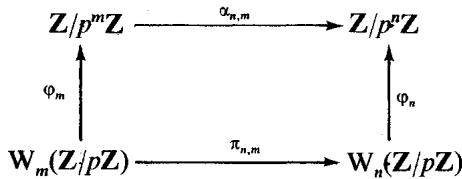
\includegraphics[keepaspectratio]{images/part001_40a15710.jpg}}

是交换的。由此，\(\varphi = \varprojlim \varphi_n\) 是从 \(\mathbf{W}(\mathbf{Z}/p\mathbf{Z}) = \varprojlim \mathbf{W}_n(\mathbf{Z}/p\mathbf{Z})\) 到 \(\mathbf{Z}_p = \varprojlim \mathbf{Z}/p^n\mathbf{Z}\) 的拓扑环同构（III，第 2 节第 12 号例 3）。

设 \(m\)、\(n\) 为两个 \(\geqslant 1\) 的整数。按构造，有加法群的正合序列

\[
0 \longrightarrow \mathrm{W} (\mathrm{A}) \xrightarrow {\mathrm{V} ^ {m}} \mathrm{W} (\mathrm{A}) \xrightarrow {\pi_ {m}} \mathrm{W} _ {m} (\mathrm{A}) \longrightarrow 0.\tag{E}
\]

通过取商，W(A) 的加法群自同态 \(V^{n}\) 定义了同态 \(V_{m}^{n}\)，其从 \(W_{m}(A)\) 的加法群到 \(W_{m+n}(A)\) 的加法群。换言之，有交换图

\pandocbounded{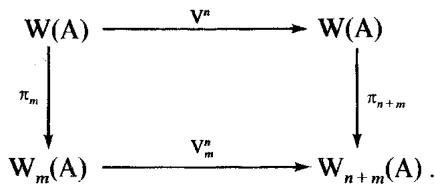
\includegraphics[keepaspectratio]{images/part001_7fe9268c.jpg}}

通过取商，由正合序列 (E) 得到正合序列

\[
0 \longrightarrow \mathrm{W} _ {m} (\mathrm{A}) \xrightarrow {\mathrm{V} _ {m} ^ {n}} \mathrm{W} _ {n + m} (\mathrm{A}) \xrightarrow {\pi_ {n , n + m}} \mathrm{W} _ {n} (\mathrm{A}) \longrightarrow 0.\tag{E'}
\]

有

\[
\mathrm{V} _ {m} ^ {n} [ a _ {0}, \dots , a _ {m - 1} ] = [ \underbrace {0 , \dots , 0} _ {n \text {   times }}, a _ {0}, \dots , a _ {m - 1} ],\tag{45}
\]

对每个元素 \([a_0, \ldots, a_{m-1}]\)，只要它属于 \(\mathbf{W}_m(\mathbf{A})\)，均成立。

根据第 5 节命题 3 的 c)，对 W(A) 中的所有 a，有 FV \(^{m+1}\) (a) = p.V \(^{m}\) (a)，从而 F(V \(_{m+1}\) (A)) ⊂ V \(_{m}\) (A)。对 n 归纳可知，F \(^{n}\) 将 V \(_{n+m}\) (A) 映入 V \(_{m}\) (A)，因而通过取商定义了环同态 F \(^{n}\) :W \(_{n+m}\) (A) → W \(_{m}\) (A)。按构造，有交换图

\pandocbounded{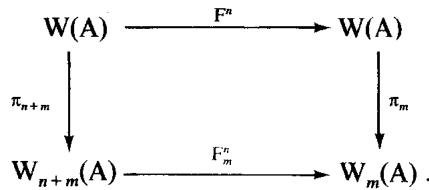
\includegraphics[keepaspectratio]{images/part001_14e9ec0a.jpg}}

回忆（第 3 节），多项式 \(\mathbf{F}_i\) 属于 \(\mathbf{Z}[\mathbf{X}_0, \ldots, \mathbf{X}_{i+1}]\)，对每个整数 \(i \geqslant 0\) 均如此；因此，同态 \(\mathbf{F}_m^1\) 从 \(\mathbf{W}_{m+1}(\mathbf{A})\) 到 \(\mathbf{W}_m(\mathbf{A})\)，可明确写为：

\[
\mathrm{F} _ {m} ^ {1} \left[ a _ {0}, \dots , a _ {m} \right] = \left[ \mathrm{F} _ {i} \left(a _ {0}, \dots , a _ {i + 1}\right) \right] _ {0 \leqslant i <   m}.\tag{46}
\]

设 \(\boldsymbol{a} \in \mathrm{W}_{m}(\mathbf{A})\)、\(\boldsymbol{a}' \in \mathrm{W}_{m}(\mathbf{A})\)，以及 \(\boldsymbol{b} \in \mathrm{W}_{m+1}(\mathbf{A})\)。下列公式由第 5 节命题 3 通过取商得到：

\begin{enumerate}
\def\labelenumi{(\arabic{enumi})}
\setcounter{enumi}{46}
\tightlist
\item
\end{enumerate}

\[
\mathrm{F} _ {m} ^ {1} \left(\mathrm{V} _ {m} ^ {1} (\boldsymbol {a})\right) = p. \boldsymbol {a}\tag{48}
\]

\[
\mathrm{V} _ {m} ^ {1} (a \times \mathrm{F} _ {m} ^ {1} (b)) = \mathrm{V} _ {m} ^ {1} (a) \times b\tag{49}
\]

\[
\mathrm{V} _ {m} ^ {1} (a) \times \mathrm{V} _ {m} ^ {1} (a ^ {\prime}) = p. \mathrm{V} _ {m} ^ {1} (a \times a ^ {\prime})\tag{50}
\]

\[
\mathrm{V} _ {m} ^ {1} (\mathrm{F} _ {m} ^ {1} (b)) = \mu_ {m + 1} \times b
\]

\((\text{其中 } \boldsymbol{\mu}_{m+1} = [0, 1, 0, ..., 0]).\)

\subsection{系数在特征为 p 的环中的 Witt 向量环}

命题 5．——设 A 为特征为 p 的环（A，V，第 2 页）。对 W(A) 中的任意元素 a、b 以及正整数 m、n，若 \(\boldsymbol{a} = (a_{n})_{n \in \mathbb{N}}\)，

\begin{enumerate}
\def\labelenumi{(\arabic{enumi})}
\setcounter{enumi}{50}
\tightlist
\item
\end{enumerate}

\[
\mathrm{F} (\boldsymbol {a}) = (a _ {n} ^ {p}) _ {n \in \mathbf {N}}\tag{52}
\]

\[
p. \boldsymbol {a} = \operatorname{VF} (\boldsymbol {a}) = \operatorname{FV} (\boldsymbol {a}) = (0, a _ {0} ^ {p}, a _ {1} ^ {p}, \dots)\tag{53}
\]

\[
\mathrm{V} ^ {m} (a) \times \mathrm{V} ^ {n} (b) = \mathrm{V} ^ {m + n} (\mathrm{F} ^ {n} (a) \times \mathrm{F} ^ {m} (b)).
\]

公式 (51) 由第 3 节例 4 得到。由此立即推出等式

\[
\operatorname{VF} (\boldsymbol {a}) = \operatorname{FV} (\boldsymbol {a}) = (0, a _ {0} ^ {p}, a _ {1} ^ {p}, \dots),
\]

且等式 \(p\) . \(a = \text{FV}(a)\) 已由第 5 节命题 3 证明，从而得到 (52)。

证明 (53)。由公式 (37)（其中以 \(V^n(\boldsymbol{b})\) 代替 \(\boldsymbol{b}\)），有

\[
\mathrm{V} ^ {m} (\boldsymbol {a}) \times \mathrm{V} ^ {n} (\boldsymbol {b}) = \mathrm{V} ^ {m} \left(\boldsymbol {a} \times \mathrm{F} ^ {m} \left(\mathrm{V} ^ {n} (\boldsymbol {b})\right)\right).\tag{54}
\]

由公式 (37) 还可推出

\[
\mathrm{V} ^ {n} \left(\mathrm{F} ^ {m} (\boldsymbol {b})\right) \times \boldsymbol {a} = \mathrm{V} ^ {n} \left(\mathrm{F} ^ {m} (\boldsymbol {b}) \times \mathrm{F} ^ {n} (\boldsymbol {a})\right).\tag{55}
\]

于是，公式 (53) 由 (54)、(55) 以及关系 \(F^{m} \circ V^{n} = V^{n} \circ F^{m}\) 得到，而后一个关系本身是 (51) 的结果。

推论．——若 m、n 为两个正整数，则有

\[
\mathrm{V} _ {m} (\mathrm{A}) \times \mathrm{V} _ {n} (\mathrm{A}) \subset \mathrm{V} _ {m + n} (\mathrm{A}).
\]

这由公式 (53) 得到，因为 \(V_{m}(A)\) 是 \(V^{m}:W(A)\to W(A)\) 的像。

命题 6．——设 A 为一个环。

\begin{enumerate}
\def\labelenumi{\alph{enumi})}
\item
  对每个整数 \(k \geqslant 1\)，都有 \((\mathrm{V}_1(\mathrm{A}))^k = p^{k-1} \cdot \mathrm{V}_1(\mathrm{A})\)。
\item
  假设 A 是特征为 p 的环。在环 W(A) 上，V₁(A)-进拓扑与 p-进拓扑重合，并且二者都比乘积拓扑 ℰ 精细（参见第 6 节）。环 W(A) 关于 p-进拓扑是分离且完备的。
\end{enumerate}

证明 \(a\)：对 \(k\) 归纳。当 \(k = 1\) 时显然成立。设 \(k \geqslant 2\)。根据归纳假设，有 \(\mathrm{V}_{1}(\mathrm{A})^{k-1} = p^{k-2} \cdot \mathrm{V}_{1}(\mathrm{A})\)，从而 \(\mathrm{V}_{1}(\mathrm{A})^{k} = p^{k-2} \cdot (\mathrm{V}_{1}(\mathrm{A}))^{2}\)。但由第 5 节命题 3 的 \(d\)、公式 (31)，有 \((\mathrm{V}_{1}(\mathrm{A}))^{2} = p \cdot \mathrm{V}_{1}(\mathrm{A})\)，故得 \(a\)。

现在假设 A 具有特征 p。由于有

\[
p. \mathrm{W} (\mathrm{A}) = \mathrm{VF} (\mathrm{W} (\mathrm{A})) \subset \mathrm{V} _ {1} (\mathrm{A}) \quad (\text { formula (52) }),
\]

由 \(a\) 得到包含关系 \(p^{k} \cdot \mathbf{W}(\mathbf{A}) \subset (\mathbf{V}_{1}(\mathbf{A}))^{k} \subset p^{k-1} \cdot \mathbf{W}(\mathbf{A})\)，并由命题 5 的推论得到包含关系 \((\mathbf{V}_{1}(\mathbf{A}))^{k} \subset \mathbf{V}_{k}(\mathbf{A})\)，对每个整数 \(k \geqslant 1\) 均如此。由此得到 \(b\) 的第一条断言。

设 \(k\) 为一个 \(\geqslant 1\) 的整数。根据公式 (52)，W(A) 的理想 \(p^{k}\) . W(A) 是 W(A) 中元素 \(\boldsymbol{a} = (a_{n})_{n \in \mathbf{N}}\) 所成的集合，其中元素满足 \(a_{n} = 0\)（\(n < k\)）且 \(a_{n} \in A^{p^{k}}\)（\(n \geqslant k\)）。因此它关于拓扑 \(\mathcal{G}\) 是闭的。由于 W(A) 关于拓扑 \(\mathcal{G}\) 分离且完备，而 W(A) 的理想 \(p^{k}\) . W(A)（对 \(k \geqslant 1\)）构成 W(A) 中 \(p\)-进拓扑的 0 的邻域基，故环 W(A) 关于 \(p\)-进拓扑分离且完备（TG，III，第 26 页，命题 10 的推论 1）。

命题 7．——设 A 为特征为 p 的完美环。

\begin{enumerate}
\def\labelenumi{\alph{enumi})}
\item
  对 W(A) 的每个元素 \(\boldsymbol{a} = (a_{n})_{n \in \mathbb{N}}\)，通项为 \(p^{n}\tau(a_{n}^{p^{-n}})\) 的级数在 W(A) 中收敛，且其和为 a。
\item
  在 \(\mathbf{W}(\mathbf{A})\) 上，\(\mathbf{V}_1(\mathbf{A})\)-进拓扑、\(p\)-进拓扑和拓扑 \(\mathcal{C}\) 重合。更准确地说，有 \(\mathbf{V}_n(\mathbf{A}) = p^n\) . \(\mathbf{W}(\mathbf{A}) = (\mathbf{V}_1(\mathbf{A}))^n\)，对每个整数 \(n \geqslant 0\) 均成立。特别地，\(\Phi_0\) 定义了从 \(\mathbf{W}(\mathbf{A})/p\) . \(\mathbf{W}(\mathbf{A})\) 到 \(\mathbf{A}\) 的同构。
\end{enumerate}

根据定义（A，V，第 5 页），映射 \(a \mapsto a^{p}\) 是环 A 的自同构。因此由命题 5，F 是环 W(A) 的自同构，并且对每个 \(n \in \mathbf{N}\)，有

\[
p ^ {n}. \mathrm{W} (\mathrm{A}) = \mathrm{V} ^ {n} \mathrm{F} ^ {n} (\mathrm{W} (\mathrm{A})) = \mathrm{V} ^ {n} (\mathrm{W} (\mathrm{A})) = \mathrm{V} _ {n} (\mathrm{A}).
\]

特别地，有 \((\mathbf{V}_1(\mathbf{A}))^n = (p.\mathbf{W}(\mathbf{A}))^n = p^n.\mathbf{W}(\mathbf{A})\)。断言 \(b)\) 由此得到。由命题 5，有

\[
p ^ {n} \cdot \tau (a _ {n} ^ {p ^ {- n}}) = \mathrm{V} ^ {n} \mathrm{F} ^ {n} \tau (a _ {n} ^ {p ^ {- n}}) = \mathrm{V} ^ {n} \tau (a _ {n}),
\]

从而由第 6 节命题 4 得到断言 a)。

命题 8．——设 A 为特征为 p 的域。环 W(A) 是一个局部整环，分离且完备，其极大理想为 V₁(A)，剩余域同构于 A。若域 A 是完美的，则环 W(A) 是一个离散赋值环，其极大理想为 p.W(A)。

同态 \(\Phi_{0}\) 定义了从 W(A)/V \(_{1}\) (A) 到 A 的同构（第 7 节例 1）。因此，V \(_{1}\) (A) 是 W(A) 的极大理想。由于环 W(A) 关于 V \(_{1}\) (A)-进拓扑分离且完备，它是一个局部环，极大理想为 V \(_{1}\) (A)（命题 6 的 b)，以及 III，第 2 节第 13 号命题 19）。

设 \(\pmb{a}\) 和 \(\pmb{b}\) 是 \(\mathbf{W}(\mathbf{A})\) 的两个非零元素。存在整数 \(m \geqslant 0\) 和 \(n \geqslant 0\)，以及元素 \(\pmb{a}' = (a_n')_{n \in \mathbb{N}}\) 和 \(\pmb{b}' = (b_n')_{n \in \mathbb{N}}\)，它们属于 \(\mathbf{W}(\mathbf{A})\)，使得 \(\pmb{a} = \mathbf{V}^m(\pmb{a}')\)、\(\pmb{b} = \mathbf{V}^n(\pmb{b}')\)，且 \(a_0'\)、\(b_0'\) 是 \(\mathbf{A}\) 中的非零元素。于是，下标为 \(m + n\) 的 \(\pmb{a} \times \pmb{b}\) 的分量等于下标为 0 的 \(\mathbf{F}^n(\pmb{a}') \times \mathbf{F}^m(\pmb{b}')\) 的分量（公式 (53)），即等于 \(a_0'^{p^n} b_0'^{p^m}\)（公式 (51) 及第 3 节例 2）。因此 \(\pmb{a} \times \pmb{b}\) 非零，且 \(\mathbf{W}(\mathbf{A})\) 是整环。

若域 A 是完美的，则极大理想 \(V_{1}(A)\) 属于 \(W(A)\)，并等于 p.\(W(A)\)

（命题 7 的 b)），从而 W(A) 是一个离散赋值环（VI，第 3 节第 6 号命题 9 的 c)）。

备注．——1) 设 A 为特征为 p 的域。可以证明，环 W(A) 是诺特环当且仅当 A 是完美的（第 43 页习题 9）。

\begin{enumerate}
\def\labelenumi{\arabic{enumi})}
\setcounter{enumi}{1}
\tightlist
\item
  设 A 为特征为 p 的环。由命题 5，有公式
\end{enumerate}

\[
\mathrm{F} _ {m} ^ {n} [ a _ {0}, \dots , a _ {n + m - 1} ] = [ a _ {0} ^ {p ^ {n}}, \dots , a _ {m - 1} ^ {p ^ {n}} ]
\]

\[
p ^ {n} \cdot [ a _ {0}, \dots , a _ {n + m - 1} ] = [ \underbrace {0 , \dots , 0} _ {n \text {   times }}, a _ {0} ^ {p ^ {n}}, \dots , a _ {m - 1} ^ {p ^ {n}} ]
\]

对每个 Witt 向量 \([a_0, \dots, a_{n+m-1}]\)，其长度为 \(n + m\)，均成立。

事实上，映射 \(F:W(A)\to W(A)\) 使我们能够通过对 \(V_{m}(A)\) 取商来定义映射 \(\overline{F}_{m}:W_{m}(A)\to W_{m}(A)\)。有公式

\[
\overline {{{{\mathrm{F}}}}} _ {m} \left[ a _ {0}, \dots , a _ {m - 1} \right] = \left[ a _ {0} ^ {p}, \dots , a _ {m - 1} ^ {p} \right].
\]

映射 \(V_{m}^{1} \circ \overline{F}_{m}\) 和 \(\overline{F}_{m+1} \circ V_{m}^{1}\) 从 \(W_{m}(A)\) 到 \(W_{m+1}(A)\)，彼此相等，并且通过取商由 \(W_{m+1}(A)\) 中乘以 p 得到。

\section{COHEN 环}

本节中，p 表示素数。

\subsection{\texorpdfstring{\(p\)-环}{p-环}}

定义 1．——若环 C 的理想 pC 是极大理想，且 C 关于 pC-进拓扑分离且完备，则称 C 为 p-环。

设 C 为一个环；若 \(p1_{C}\) 是幂零的且 C 的理想 pC 是极大理想，则 C 是 p-环，因为 C 的 pC-进拓扑是离散的。特别地，每个特征为 p 的域都是 p-环。

命题 1．——设 C 为一个 p-环。

\begin{enumerate}
\def\labelenumi{\alph{enumi})}
\item
  环 C 是局部环，极大理想为 pC。
\item
  假设 \(p1_{\mathbb{C}}\) 是幂零的。设 \(d\) 是满足 \(p^{d}1_{\mathbb{C}} = 0\) 的最小正整数。\(\mathbb{C}\) 的理想形如 \(p^{k}\mathbb{C}\)，其中 \(0 \leqslant k \leqslant d\)，且有 \(p^{k}\mathbb{C} \neq p^{l}\mathbb{C}\)，这里 \(k\)、\(l\) 是满足 \(0 \leqslant k \leqslant d, 0 \leqslant l \leqslant d\) 的两个不同整数。\(\mathbb{C}\)-模 \(\mathbb{C}\) 的长度为 \(d\)。
\item
  假设 \(p1_{\mathbb{C}}\) 不是幂零的。则 C 是离散赋值环，其剩余域的特征为 \(p\)，其分式域的特征为 0。形如 \(p^{n}\mathbf{C}\)（\(n \in \mathbf{N}\)）的理想两两不同；它们构成 C 的全部非零理想。C-模 C 的长度不是有限的。
\end{enumerate}

断言 \(a)\) 由 III，第 2 节第 13 号命题 19 得到。

由假设，\(\bigcap_{n\geqslant 0}p^{n}\mathbf{C} = \{0\}\)。设 \(x\neq 0\) 属于 \(\mathbf{C}\)；存在整数 \(n\geqslant 0\)，使得 \(x\in p^n\mathbf{C}, x\notin p^{n + 1}\mathbf{C}\)；因而存在元素 \(y\)，它属于 \(\mathbf{C}\)，且 \(x = p^n y\)；由于 \(y\) 不属于 \(p\mathbf{C}\)，故 \(y\) 可逆。

假设 \(p1_{\mathbb{C}}\) 不是幂零的。若 \(x\)、\(x'\) 是 C 的两个非零元素，则存在两个整数 \(n \geqslant 0\)、\(n' \geqslant 0\) 以及 C 的两个可逆元素 \(y\)、\(y'\)，使得 \(x = p^n y\)、\(x' = p^{n'} y'\)。于是 \(xx' = p^{n+n'} yy' \neq 0\)，故 C 是整环。由于 C 是局部环但不是域，且 C 的极大理想 \(m_{\mathbb{C}} = p\mathbb{C}\) 是主理想，C 是离散赋值环（VI，第 3 节第 6 号命题 9）。于是根据上引文献命题 8，C 的非零理想形如 \(p^n\mathbb{C}\)，且两两不同。特别地，环 C 不是阿廷环，因而 C-模 C 的长度不是有限的。C 的剩余域 C/pC 的特征为 \(p\)。设 C 的分式域的特征为 \(q\)。有 \(p1_{\mathbb{C}} \neq 0\)，从而 \(p \neq q\)。此外，若 \(q\) 非零，则有 \(q1_{\mathbb{C}} = 0\)，从而 C/pC 的特征为 \(q \neq p\)，这是荒谬的。这就证明了 \(c\)。

假设 \(p1_{C}\) 是幂零的。设 \(d\) 是满足 \(p^{d}1_{C} = 0\) 的最小正整数。我们有理想序列

\[
\mathrm{C} \supset p \mathrm{C} \supset p ^ {2} \mathrm{C} \supset \dots \supset p ^ {d - 1} \mathrm{C} \supset p ^ {d} \mathrm{C} = \{0 \}.\tag{E}
\]

若 \(k\) 是满足 \(0 \leqslant k < d\) 且 \(p^k\mathbf{C} = p^{k+1}\mathbf{C}\) 的整数，则可推出

\[
p ^ {d - k - 1} p ^ {k} \mathrm{C} = p ^ {d - k - 1} p ^ {k + 1} \mathrm{C} = \{0 \}
\]

这与假设 \(p^{d-1}1_{\mathbf{C}} \neq 0\) 矛盾。因此，序列 (E) 的元素两两不同。设 \(\mathfrak{a}\) 是 C 的一个理想，令 \(k\) 为满足 \(\mathfrak{a} \supset p^k\mathbf{C}\) 的最小正整数。设 \(x\) 是非零元素，属于 \(\mathfrak{a}\)；我们已经看到，\(x\) 形如 \(p^m u\)，其中 \(m \geqslant 0\)，且 \(u\) 在 C 中可逆。因此 \(p^m\mathbf{C} \subset \mathfrak{a}\)，从而 \(m \geqslant k\)，最终 \(x \in p^k\mathbf{C}\)。总之，\(\mathfrak{a} = p^k\mathbf{C}\)。于是序列 (E) 是 C-模 C 的 Jordan–Hölder 序列，其长度为 \(d\)。

推论 1．——若 p-环 C 是整环，则它是离散赋值环，或是特征为 p 的域。

设 C 是整环。若 \(p1_{\mathbf{C}}\) 是幂零的，则 \(p1_{\mathbf{C}} = 0\)，而 \(\{0\}\) 是 C 的极大理想，故 C 是特征为 \(p\) 的域。若 \(p1_{\mathbf{C}}\) 不是幂零的，则由命题 1 的 c)，C 是离散赋值环。

推论 2．——设 C 为 p-环，且 a 是 C 中异于 C 的理想。环 C/a 是 p-环。

不妨设 \(\mathfrak{a} \neq \{0\}\)。于是存在整数 \(i \geqslant 1\)，使得 \(\mathfrak{a} = p^i\mathrm{C}\)；理想 \(p\mathrm{C} / \mathfrak{a}\) 是 \(\mathrm{C} / \mathfrak{a}\) 的极大理想，且 \(p^i1_{\mathrm{C} / \mathfrak{a}} = 0\)，故 \(\mathrm{C} / \mathfrak{a}\) 是一个 \(p\) -环。

设 C 为一个 \(p\) -环。称 C 的长度为 \(l(\mathbf{C})\)，并将其定义为 \(\overline{\mathbf{R}}\) 中所有满足 \(n \geqslant 1\) 且 \(p^{n-1}1_{\mathbf{C}} \neq 0\) 的整数所成集合的上确界。当 \(l(\mathbf{C})\) 有限时，它就是 C-模 C 的长度；当 \(l(\mathbf{C})\) 等于 \(+\infty\) 时，C-模 C 的长度不是有限的（命题 1）。

例．——1) 对每个整数 \(n \geqslant 1\)，环 \(\mathbf{Z}/p^{n}\mathbf{Z}\) 都是一个 \(p\)-环，长度为 \(n\)。环 \(\mathbf{Z}_{p}\) 是 \(p\)-进整数环，也是无限长度的 \(p\)-环。

\begin{enumerate}
\def\labelenumi{\arabic{enumi})}
\setcounter{enumi}{1}
\tightlist
\item
  设 K 为特征为 p 的完美域。根据第 1 节第 8 号命题 8，Witt 向量环 W(K) 是无限长度的 p-环。映射 \((a_{n})_{n\in\mathbf{N}} \mapsto a_{0}\) 通过取商诱导出从 W(K)/pW(K) 到域 K 的同构（上引文献命题 7）。对每个整数 \(n \geqslant 1\)，环
\end{enumerate}

\[
\mathrm{W} _ {n} (\mathrm{K}) = \mathrm{W} (\mathrm{K}) / p ^ {n} \mathrm{W} (\mathrm{K})
\]

是长度为 n 的 p-环。

命题 2．——设 C 和 C' 是两个 p-环，且 \(u\) 是从 C 到 C' 的同态。设 \(v\) 是从 \(\kappa_{\mathbf{C}} = \mathbf{C} / p\mathbf{C}\) 到 \(\kappa_{\mathbf{C}'} = \mathbf{C}' / p\mathbf{C}'\) 的同态，它由 u 通过取商诱导。

\begin{enumerate}
\def\labelenumi{\alph{enumi})}
\item
  有 \(l(\mathbf{C}) \geqslant l(\mathbf{C}')\)，且 u 为单射当且仅当 \(l(\mathbf{C}) = l(\mathbf{C}')\)。
\item
  u 为满射的充要条件是 v 为同构。
\item
  u 为同构的充要条件是 v 为同构且 \(l(\mathbf{C}) = l(\mathbf{C}')\)。
\end{enumerate}

令 \(n \geqslant 1\) 为整数。有 \(u(p^{n-1}1_{\mathbf{C}}) = p^{n-1}1_{\mathbf{C}'}\)，因此关系 \(p^{n-1}1_{\mathbf{C}'} \neq 0\) 蕴含 \(p^{n-1}1_{\mathbf{C}} \neq 0\)，并且当 \(u\) 为单射时与之等价。所以 \(l(\mathbf{C}') \leqslant l(\mathbf{C})\)，且当 \(u\) 为单射时等号成立。若 \(u\) 不是单射，则存在整数 \(i < l(\mathbf{C})\)，使得 \(u\) 的核是理想 \(p^i\mathbf{C}\)（属于 \(\mathbf{C}\)）；于是 \(p^i1_{\mathbf{C}'} = 0\)，从而 \(l(\mathbf{C}') \leqslant i\)。这就证明了 \(a\)。

由于 \(\kappa_{\mathrm{C}}\) 和 \(\kappa_{\mathrm{C}'}\) 是域，同态 \(v\) 是单射。若 \(u\) 是满射，则 \(v\) 也是满射，因而是同构。反之，设 \(v\) 是满射。于是对于每个整数 \(n \geqslant 0\)，映射 \(v_{n}: p^{n}\mathrm{C}/p^{n+1}\mathrm{C} \to p^{n}\mathrm{C}'/p^{n+1}\mathrm{C}'\) 由 \(u\) 得到且是满射。由于 C 关于 \(p\mathrm{C}\)-进滤子完备，而 \(\mathbf{C}'\) 关于 \(p\mathbf{C}'\)-进滤子分离，根据 III，§ 2，第 8 号的定理 1 的推论 2，\(u\) 是满射。这就证明了 \(b\)。

最后，c) 由 a) 和 b) 得出。

命题 3．——设 \((\mathbf{C}_{n}, \pi_{n,m})\) 是相对于指标集 N 的环的射影系统。假设 \(\mathbf{C}_{n}\) 对所有 \(n \in \mathbf{N}\) 都是 p-环，且同态 \(\pi_{n,m}\) 都是满射。则 \(C = \varprojlim C_{n}\) 是 p-环，并且对于所有 \(n \in \mathbf{N}\)，典范同态 \(\pi_{n}: C \to C_{n}\) 是满射，并诱导出从 \(\kappa_{C}\) 到 \(\kappa_{C_{n}}\) 的同构。

由于映射 \(\pi_{n,m}\) 是满射，映射 \(\pi_n\) 也具有同样性质（E，III，p. 58，命题 5）。我们来证明 C 是一个 \(p\)-环。令 \(d_n\) 为 \(\mathbf{C}_n\) 的长度。根据命题 2 a)，序列 \(d_n\)（其元素属于 \(\mathbf{N} \cup \{+\infty\}\)）是递增的；若它是平稳的，则存在整数 \(n_0\)，使得 \(\pi_{n,m}\) 是从 \(\mathbf{C}_m\) 到 \(\mathbf{C}_n\) 的同构，当 \(n_0 \leqslant n \leqslant m\) 时，于是 C 同构于 \(\mathbf{C}_{n_0}\)，是一个 \(p\)-环。

因此只需考虑每个 \(d_{n}\) 都有限且序列 \((d_{n})\) 趋于 \(+\infty\) 的情形。赋予环 C 平凡滤子（III，§ 2，第 1 号，例 5）。对于 \(n\in\mathbf{N}\)，令 \(\mathbf{I}_{n}\) 为 \(\pi_{n}\) 的核；置 \(\mathbf{I}_{n}=\mathbf{C}\)（当 \(n<0\) 时）。令 E 表示带有滤子 \((\mathbf{I}_{n})_{n\in\mathbf{Z}}\) 的 C-模 C。它是分离且完备的，因为拓扑 \(\mathcal{G}\) 由滤子 \((\mathbf{I}_{n})_{n\in\mathbf{Z}}\) 定义，正是各 \(\mathbf{C}_{n}\) 上离散拓扑的射影极限拓扑。

令 \(k\) 为满足 \(\geqslant 1\) 的整数。有 \(p^{k}\mathrm{C} \subset \varprojlim (p^{k}\mathrm{C}_{n})\)（E，III，p. 55，公式（9））。反之，若 \(x = (x_{n})_{n \in \mathbb{N}} \in \varprojlim (p^{k}\mathrm{C}_{n})\)，并置 \(\mathrm{X}_{n} = \{y \in \mathrm{C}|\pi_{n}(p^{k}y) = x_{n}\}\)，则序列 \((\mathrm{X}_{n})_{n \in \mathbb{N}}\) 是 E 的非空闭仿射子集的递减序列。由于 \(\mathrm{E / I}_{n}\) 是阿廷 C-模，\(\mathrm{X}_{n}\) 的交非空（III，§ 2，第 7 号，命题 7）；对于每个 \(z \in \bigcap_{n \in \mathbb{N}} \mathrm{X}_{n}\)，都有 \(p^{k}z = x\)。因此我们证明了 \(p^{k}\mathrm{C} = \varprojlim p^{k}\mathrm{C}_{n}\)。

对于每个整数 \(k \geqslant 1\)。特别地，C 的理想 \(p^{k}\text{C}\) 关于拓扑 \(\mathcal{G}\) 是闭的。在 C 上，\(p\)-进拓扑比拓扑 \(\mathcal{G}\) 更细，因为有 \(p^{d_{n}}\text{C} \subset \text{I}_{n}\)。于是根据 TG，III，p. 26，命题 10 的推论 1，C 关于 \(p\text{C}\)-进拓扑是分离且完备的。此外，有 \(p\text{C} = \varprojlim p\text{C}_{n} = \pi_{0}^{-1}(p\text{C}_{0})\)，所以从 C/pC 到 \(\text{C}_{0}/p\text{C}_{0}\) 的满射同态（由 \(\pi_{0}\) 得到）是同构。这说明 C 的理想 \(p\text{C}\) 是极大理想，因而 C 是一个 \(p\)-环。命题 3 的最后一个断言由命题 2 b) 得出。

\subsection{科恩环}

定义 2．——设 A 是一个分离且完备的局部环，其剩余域的特征为 p。称 A 的一个子环 C 为 A 的一个科恩子环，如果 C 是 p-环且满足 \(\mathbf{A} = \mathfrak{m}_{\mathbf{A}} + \mathbf{C}\)（即 \(\mathbf{A}/\mathfrak{m}_{\mathbf{A}} = \mathbf{C}/(\mathfrak{m}_{\mathbf{A}} \cap \mathbf{C})\)）。

若 C 是 A 的一个科恩子环，则 C 的理想 \(m_{A} \cap C\) 是极大理想，因而等于 pC。所以从 \(\kappa_{C} = C/pC\) 到 \(\kappa_{A} = A/m_{A}\) 的典范映射是域同构。

例．——设 C 是 p-环。形式幂级数环 \(A = C[[T_{1}, \ldots, T_{n}]]\) 是一个诺特局部环，分离且完备，其极大理想由序列 (p, T₁, \ldots, Tₙ) 生成。显然 C 是 A 的一个科恩子环。特别地，当 C 等于 Zₚ、Z/pⁿZ 或特征为 p 的域时也适用。

定理 1．— 设 A 是一个局部环，分离且完备，其剩余域 k 的特征为 p。设 π 是从 A 到 k 的典范映射，并设 S 是 A 的一个子集，使 π 将 S 双射到 k 的一个 p-基上（A，V，p. 95）。

\begin{enumerate}
\def\labelenumi{\alph{enumi})}
\item
  存在唯一一个包含 S 的 A 的科恩子环 C。
\item
  A 的子环 C 是闭的，且 C 上的 \(p\)C-进拓扑由 A 的 \(m_{A}\)-进拓扑诱导。
\item
  A 的每个包含 S 且满足 \(A = A' + m_{A}\) 的闭子环 A' 都包含 C。
\end{enumerate}

\begin{enumerate}
\def\labelenumi{\Alph{enumi})}
\tightlist
\item
  特例：\(\mathfrak{m}_{\mathbf{A}}\) 是幂零的
\end{enumerate}

令 \(n\) 为满足 \(\mathfrak{m}_{\mathbf{A}}^{n+1}=\{0\}\) 的正整数。若 \(\Phi_{n}\) 是第 \(n\) 个 Witt 多项式（§ 1，第 1 号），则映射 \(u:[a_{0},..., a_{n}]\mapsto\Phi_{n}(a_{0},..., a_{n})\) 是从 \(\mathbf{W}_{n+1}(\mathbf{A})\) 到 \(\mathbf{A}\) 的环同态（§ 1，第 7 号）。令 \(\mathbf{B}_{n}\) 为 \(u\) 的像，并令 \(\mathbf{C}_{n}\) 为 \(\mathbf{A}\) 的由 \(\mathbf{B}_{n}\cup\mathbf{S}\) 生成的子环。

引理 1．——设 A' 是包含 S 的 A 的一个子环。A' 包含 \(\mathbf{C}_{n}\) 的充要条件是 \(A' + m_{A} = A\)。

有 \(pA \subset m_A\)，且 \(B_n\) 由形如 \(a_0^{p^n} + pa_1^{p^{n-1}} + \cdots + p^n a_n\) 的元素组成，其中 \(a_0, \ldots, a_n\) 属于 A。因此 \(\pi(B_n) = k^{p^n}\)，从而 \(\pi(C_n) = k^{p^n}[\pi(S)]\)。但由于 \(\pi(S)\) 是一个 \(p\)-基（属于 \(k\)），有 \(k = k^{p^n}[\pi(S)]\)（A，V，p. 96），从而 \(\pi(C_n) = k\)，即 \(C_n + m_A = A\)。

设 A' 是包含 S 的 A 的一个子环。若 A' 包含 \(C_{n}\)，则有

\[
\mathrm{A} ^ {\prime} + \mathrm{m} _ {\mathrm{A}} \supset \mathrm{C} _ {n} + \mathrm{m} _ {\mathrm{A}} = \mathrm{A}, \quad \mathrm{whence} \quad \mathrm{A} ^ {\prime} + \mathrm{m} _ {\mathrm{A}} = \mathrm{A}.
\]

反之，设 \(\mathbf{A}' + \mathfrak{m}_{\mathbf{A}} = \mathbf{A}\)。令 \(a_0, \ldots, a_n\) 为 \(\mathbf{A}\) 中的元素；根据假设，存在元素 \(a_0', \ldots, a_n'\) 属于 \(\mathbf{A}'\)，使得 \(a_i \equiv a_i'\) 模 \(\mathfrak{m}_{\mathbf{A}}\)（对 \(0 \leqslant i \leqslant n\)）。根据 § 1 第 1 号的命题 1 及假设 \(\mathfrak{m}_{\mathbf{A}}^{n+1} = \{0\}\)，有 \(\Phi_n(a_0, \ldots, a_n) = \Phi_n(a_0', \ldots, a_n') \in \mathbf{A}'\)，从而 \(\mathbf{B}_n \subset \mathbf{A}'\)。由于 \(\mathbf{C}_n\) 是由 \(\mathbf{B}_n \cup \mathbf{S}\) 生成的环，有 \(\mathbf{C}_n \subset \mathbf{A}'\)。

在所有包含 S 且满足 \(A' + m_{A} = A\) 的 A 的子环 A' 所成的集合中，根据引理 1 存在一个最小元素 C，并且有 \(C_{n} = C\)，对于每个整数 \(n \geqslant 0\) 满足 \(m_{A}^{n+1} = \{0\}\) 时均如此。

按构造有 \(C + m_A = A\)，且 \(p1_C\) 是幂零的。显然 \(pC \subset C \cap m_A\)，因此下面的引理 2 表明 \(pC\) 是 \(C\) 的极大理想，从而 \(C\) 是 \(A\) 的一个科恩子环。

引理 2．——有 \(C \cap m_{A} \subset pC\)。

取整数 \(m \geqslant 1\)，使得 \(\mathfrak{m}_{\mathbf{A}}^{m} = \{0\}\)，从而 \(\mathbf{C} = \mathbf{C}_{m} = \mathbf{C}_{m-1}\)。令 \(\Lambda\) 为 \(\mathbf{N}^{(\mathbf{S})}\) 的一部分，它由有限支撑的整数族 \((\alpha_{s})_{s \in \mathbf{S}}\) 组成，并满足 \(0 \leqslant \alpha_{s} < p^{m}\)，对每个 \(s \in \mathbf{S}\) 均如此。由于 \(\mathbf{B}_{m}\) 包含 \(s^{p^{m}} = \Phi_{m}(s, 0, ..., 0)\)（对每个 \(s \in \mathbf{S}\)），单项式 \(Z_{\alpha} = \prod_{s \in \mathbf{S}} s^{\alpha_{s}}\)（其中 \(\alpha\) 遍历 \(\Lambda\)）生成 \(\mathbf{C}_{m}\)，作为 \(\mathbf{B}_{m}\)-模。此外，根据公式

\[
\Phi_ {m} (a _ {0}, \dots , a _ {m}) = a _ {0} ^ {p ^ {m}} + p \Phi_ {m - 1} (a _ {1}, \dots , a _ {m}),
\]

 \(B_{m}\) 的每个元素都形如 \(a^{p^{m}} + pb\)，其中 \(a \in A\) 且 \(b \in B_{m-1}\)。因此 \(C = C_{m}\) 的每个元素都形如

\[
x = \sum_ {\alpha \in \Lambda} c _ {\alpha} ^ {p ^ {m}} Z _ {\alpha} + p y\tag{1}
\]

其中 \(c_{\alpha} \in \mathbf{A}\) 对每个 \(\alpha \in \Lambda\) 均成立，且 \(y \in \mathbf{C}_{m-1} = \mathbf{C}\)。若 \(x\) 属于 \(\mathbf{C} \cap \mathfrak{m}_{\mathbf{A}}\)，则有 \(\pi(x) = 0\)，从而 \(\sum_{\alpha \in \Lambda} \pi(c_{\alpha})^{p^m} \pi(Z_{\alpha}) = 0\)。由于 \(\pi(\mathbf{S})\) 是一个 \(p\)-基（属于 \(k\)），根据 A，V，p. 96，有 \(\pi(c_{\alpha}) = 0\) 对每个 \(\alpha \in \Lambda\) 均成立。于是 \(c_{\alpha} \in \mathfrak{m}_{\mathbf{A}}\)，从而 \(c_{\alpha}^m = 0\)，当然也有 \(c_{\alpha}^{p^m} = 0\)。由 (1) 得 \(x = py\)，从而得到引理 2。

有 \(p^m\mathbf{C} = \mathfrak{m}_{\mathbf{A}}^m = \{0\}\)（当 \(m\) 足够大时），所以断言 \(b)\) 显然成立。断言 \(c)\) 由引理 1 得出。若 \(\mathbf{C}'\) 是包含 S 的 A 的一个科恩子环，则根据引理 1 有 \(\mathbf{C}' \supset \mathbf{C}\)。但由于 C 到 \(\mathbf{C}'\) 的包含映射诱导出从 \(\kappa_{\mathbf{C}}\) 到 \(\kappa_{\mathbf{C}'}\) 的同构，有 \(\mathbf{C} = \mathbf{C}'\)（第 1 号，命题 2 b)），这就完成了 \(a\) 的证明。

\noindent\textbf{B) 一般情形.}\par

对于每个整数 \(n \geqslant 0\)，记 \(\mathbf{A}_n\) 为局部环 \(\mathbf{A}/\mathfrak{m}_{\mathbf{A}}^{n+1}\)，\(\mathfrak{m}_n = \mathfrak{m}_{\mathbf{A}}/\mathfrak{m}_{\mathbf{A}}^{n+1}\) 为其极大理想，并记 \(\pi_n\) 为从 A 到 \(\mathbf{A}_n\) 的典范同态。根据 A)，存在唯一的科恩子环 \(\mathbf{C}_n\)，它是 \(\mathbf{A}_n\) 的且包含 \(\pi_n(\mathbf{S})\)。当 \(0 \leqslant n \leqslant m\) 时，记 \(\pi_{n,m}\) 为从 \(\mathbf{A}_m\) 到 \(\mathbf{A}_n\) 的典范同态。根据第 1 号的命题 1 的推论 2，\(\pi_{n,m}(\mathbf{C}_m)\) 是一个 \(p\)-环；有 \(\pi_{n,m}(\mathbf{C}_m) + \mathfrak{m}_n = \mathbf{A}_n\)，所以 \(\pi_{n,m}(\mathbf{C}_m)\) 等于 \(\mathbf{C}_n\)，即 \(\mathbf{A}_n\) 的科恩子环。根据第 1 号的命题 3，子环 \(\varprojlim \mathbf{C}_n\) 位于 \(\varprojlim \mathbf{A}_n\) 中，是一个 \(p\)-环。置 \(\mathbf{C} = \bigcap_{n \in \mathbb{N}} \pi_n^{-1}(\mathbf{C}_n)\)。由于 C 是 \(\varprojlim \mathbf{C}_n\) 在同构 \(a \mapsto (\pi_n(a))_{n \in \mathbb{N}}\) 下的逆像，而该同构将 A 映到 \(\varprojlim \mathbf{A}_n\)，故 C 是 A 的闭子环，也是一个 \(p\)-环。有 \(\pi_n(\mathbf{C}) = \mathbf{C}_n\)（对每个 \(n \in \mathbb{N}\)），特别地 \(\pi_0(\mathbf{C}) = \mathbf{A}_0\)，即 \(\pi(\mathbf{C}) = k\)。所以 C 是 A 的一个科恩子环。

对于每个整数 \(n \geqslant 0\)，置 \(J_{n} = C \cap m_{A}^{n}\)。由于局部环 A 是分离的，有 \(\bigcap_{n \in \mathbb{N}} J_{n} = \{0\}\)，并且根据 \(p\)-环理想的结构（第 1 号，命题 1），C 的每个形如 \(p^{k}C\) 的理想都包含某个 \(J_{n}\)。反之，\(J_{n}\) 包含 \(p^{n}C\)。所以 C 的 \(pC\)-进拓扑由 A 的 \(m_{A}\)-进拓扑诱导。这证明了 \(b\)。

设 A' 是 A 的一个闭子环，包含 S 且满足 \(A' + m_{A} = A\)。由于 A' 是闭的，有 A' = \(\bigcap_{n\in\mathbb{N}}\pi_n^{-1}(\pi_n(A'))\)。有 \(\pi_n(A') \supset \pi_n(S)\) 且 \(\pi_n(A') + m_n = A_n\)，从而根据 A) 中已经得到的结论，\(\pi_n(A') \supset C_n\)。最后，有 \(\pi_n^{-1}(\pi_n(A')) \supset \pi_n^{-1}(C_n)\)，从而 A' ⊃ C。这证明了 c)。由此得到 A) 中所述科恩子环的唯一性。

注记．——若 \(p1_{A}\) 不是幂零的（特别地，当 A 是整环且其分式域的特征为 0 时会发生这种情况），则 C 是离散赋值环，其分式域的特征为 0。

\subsection{p-环的存在性与唯一性}

命题 4．——设 C 和 C' 是两个 p-环，满足 \(l(\mathbf{C}) \geqslant l(\mathbf{C}')\)，并设 \(\pi\)（分别为 \(\pi'\)）是从 C（分别从 C'）到 \(\kappa_{\mathbf{C}}\)（分别到 \(\kappa_{\mathbf{C}'}\)）的典范同态。设 \((x_{\lambda})_{\lambda \in \Lambda}\)（分别为 \((x_{\lambda}')_{\lambda \in \Lambda}\)）是 C（分别 C'）中的元素族，其在 \(\pi\)（分别 \(\pi'\)）下的像构成 \(\kappa_{\mathbf{C}}\)（分别 \(\kappa_{\mathbf{C}'}\)）的 p-基。设 v 是从 \(\kappa_{\mathbf{C}}\) 到 \(\kappa_{\mathbf{C}'}\) 的同构，满足 \(v(\pi(x_{\lambda})) = \pi'(x_{\lambda}')\)，对每个 \(\lambda \in \Lambda\) 均如此。于是存在唯一一个从 C 到 C' 的同态 u，使得 \(v \circ \pi = \pi' \circ u\)，且 \(u(x_{\lambda}) = x_{\lambda}'\)，对每个 \(\lambda \in \Lambda\) 均如此。它是满射。若 \(l(\mathbf{C}) = l(\mathbf{C}')\)，它是同构。

证明 u 的存在性。令 A 为 C × C' 的子环，由对 \((x, x')\) 构成，这些对满足 \(v(\pi(x)) = \pi'(x')\)。映射 \((x, x') \mapsto \pi(x)\) 是从 A 到 \(\kappa_{\mathbb{C}}\) 的满射环同态。它的核 m 等于 \(p\mathbb{C} \times p\mathbb{C}'\)，因而是 A 的极大理想。\(\mathbb{C} \times \mathbb{C}'\) 的拓扑子空间 A 在 \(\mathbb{C} \times \mathbb{C}'\) 中是闭的，因而完备；由 \(\mathbb{C} \times \mathbb{C}'\) 在 A 上诱导的拓扑是 m-进拓扑。因此 A 是以 m 为极大理想的分离且完备的局部环（III，§ 2，第 13 号，命题 19）。对于每个 \(\lambda \in \Lambda\)，根据假设有 \((x_{\lambda}, x_{\lambda}') \in A\)；若 \(\xi_{\lambda}\) 是 \((x_{\lambda}, x_{\lambda}')\) 模 m 的类，则族 \((\xi_{\lambda})_{\lambda \in \Lambda}\) 是域 A/m 的一个 \(p\)-基。根据第 2 号的定理 1，存在唯一一个 A 的科恩子环 \(\mathbb{C}''\)，包含 \((x_{\lambda}, x_{\lambda}')\)（对每个 \(\lambda \in \Lambda\)）。有 \(l(\mathbb{C}'') = l(\mathbb{C}) \geqslant l(\mathbb{C}')\)。在 \(\mathbb{C}''\) 上将 \(\mathbb{C} \times \mathbb{C}'\) 到 C 的投影限制后得到同态 \(h: \mathbb{C}'' \to \mathbb{C}\)，它诱导出从 \(\kappa_{\mathbb{C}''}\) 到 \(\kappa_{\mathbb{C}}\) 的同构。根据第 2 号的命题 2 c)，h 是从 \(\mathbb{C}''\) 到 C 的同构。同理，限制 \(h'\) 是在 \(\mathbb{C}''\) 上由 \(\mathbb{C} \times \mathbb{C}'\) 到 C' 的投影得到的满射同态，其从 \(\mathbb{C}''\) 到 C'。因此，\(\mathbb{C}''\) 是从 C 到 C' 的满射同态 \(u = h' \circ h^{-1}\) 的图像，并且显然有 \(v \circ \pi = \pi' \circ u\)，\(u(x_{\lambda}) = x_{\lambda}'\)，对每个 \(\lambda \in \Lambda\) 均如此。此外，若 \(l(\mathbb{C}) = l(\mathbb{C}')\)，u 是同构。

证明 \(u\) 的唯一性。设 \(u_{1}\) 是从 C 到 C' 的同态，满足 \(v \circ \pi = \pi' \circ u_{1}\) 且 \(u_{1}(x_{\lambda}) = x_{\lambda}'\)，对每个 \(\lambda \in \Lambda\) 均如此，并令 \(\mathbf{C}_{1}\) 为 \(u_{1}\) 的图。显然，\(\mathbf{C}_{1}\) 是 A 的科恩子环，包含 \((x_{\lambda}, x_{\lambda}')\)，对每个 \(\lambda \in \Lambda\) 均如此，从而 \(\mathbf{C}_{1} = \mathbf{C}''\)（第 2 号的定理 1），最后 \(u_{1} = u\)。

命题 5．——设 k 是特征为 p 的域，且 n 是满足 ≥ 1 的整数或 + ∞。存在一个长度为 n 且剩余域同构于 k 的 p-环。

Witt 向量环 \(\mathbf{W}(k)\) 的系数在 \(k\) 中，是分离且完备的整局部环，其剩余域同构于 \(k\)（\(\S\) 1，第 8 号，命题 8），且有 \(p\)．\(1_{\mathbf{W}(k)} \neq 0\)（同上，公式（52））。令 C 为 \(\mathbf{W}(k)\) 的一个科恩子环（第 2 号，定理 1）。则 C 是一个 \(p\)-环，长度为 +\(\infty\)，其剩余域同构于 \(k\)；若 \(n\) 是满足 \(\geqslant 1\) 的整数，则商 \(\mathrm{C}/p^{n}\mathrm{C}\) 是一个 \(p\)-环，长度为 \(n\)，其剩余域同构于 \(k\)。

注记．——1) 令 \(n\) 为满足 \(\geqslant 1\) 的整数，并令 S 为一个 \(p\)-基（属于 \(k\)）。可以证明，\(\mathbf{W}_{n}(k)\) 中由 \(\mathbf{W}_{n}(k^{p^{n}})\) 及元素 \([\xi, 0, ..., 0]\)（\(\xi \in S\)）生成的子环，是一个 \(p\)-环，长度为 \(n\)，其剩余域同构于 \(k\)（参见 p. 72，习题 10）。

\begin{enumerate}
\def\labelenumi{\arabic{enumi})}
\setcounter{enumi}{1}
\tightlist
\item
  读者将在附录中找到命题 5 的一个证明；该证明既不使用 § 1 的结果，也不使用科恩子环的存在定理（第 2 号，定理 1）。
\end{enumerate}

推论．——设 C 是长度有限的 p-环，长度为 n。存在一个无限长度的 p-环 C'，使得 C 同构于 \(C'/p^{n}C'\)。

根据命题 5，存在一个无限长度的 \(p\)-环 \(C'\)，使得 \(\kappa_{C'}\) 同构于 \(\kappa_{C}\)。于是 \(C'/p^{n}C'=C_{n}'\) 是一个 \(p\)-环，长度为 \(n\)，且域 \(\kappa_{C_{n}'}\) 同构于 \(\kappa_{C'}\)，因而同构于 \(\kappa_{C}\)。根据命题 4，环 \(C\) 与 \(C_{n}'\) 因而同构。

\subsection{乘法代表元}

命题 6．——设 C 是一个 p-环，其剩余域 k 是完美的。假设 C 的长度有限为 n（分别为无限长度）。存在唯一同构 \(u:W_{n}(k)\to C\)（分别为 \(u:W(k)\to C\)），它经过取商诱导出 k 的恒等映射。

由于 \(W_{n}(k)\)（分别为 \(W(k)\)）是剩余域为 k 且长度为 n（分别为无限长度）的 p-环（第 1 号，例 2），又由于 \(\varnothing\) 是完美域 k 的 p-基，命题 6 是第 3 号命题 4 的特例。

定理 2．——设 A 是分离且完备的局部环，k 是其剩余域，π 是从 A 到 k 的典范同态。假设 k 是特征为 p 的完美域。

\begin{enumerate}
\def\labelenumi{\alph{enumi})}
\item
  存在唯一的环同态 \(u: \mathbf{W}(k) \to \mathbf{A}\)，使得有 \(\pi(u(\boldsymbol{a})) = a_0\)，其中 \(\boldsymbol{a} = (a_n)_{n \in \mathbb{N}}\) 属于 \(\mathbf{W}(k)\)。
\item
  当 W(k) 赋予 pW(k)-进拓扑时，同态 u 是连续的，且 u 的像是 A 的唯一科恩子环。
\end{enumerate}

根据第 2 号的定理 1，存在唯一的 A 的科恩子环；记为 C。设 u 是从 W(k) 到 A 的同态，使得有 \(\pi(u(\boldsymbol{a})) = a_0\)，对每个 \(\boldsymbol{a} = (a_n)_{n \in \mathbb{N}}\)（属于 W(k)）均如此；显然 u 的像是 A 的科恩子环，因而等于 C。u 的存在性和唯一性由命题 6 得出。C 的 pC-进拓扑由 A 的 \(m_{A}\)-进拓扑诱导（第 2 号，定理 1，b)），从而 u 连续。

关于 u 的直接构造，参见 p. 70，习题 6。

命题 7．——沿用定理 2 的假设与记号。存在唯一的 A 的乘法子集 S，使 π 将 S 双射到 k。A 的元素 a 属于 S 的充要条件是：对于每个 n ∈ N，存在 A 中的元素 \(a_{n}\)，使 \(a = a_{n}^{p^{n}}\)。集合 S 正是所有形如 \(u(x, 0, 0, \ldots)\) 的元素所成的集合。

先证明 S 的唯一性。设 S 是 A 的一个乘法子集，使 \(\pi\) 将 S 双射到 k。令 T 为 A 中这样的元素所成的集合：它们对每个 \(p^{n}\)（其中 \(n \in N\)）都是 p＾n 次幂。

\begin{enumerate}
\def\labelenumi{\alph{enumi})}
\item
  有 S ⊂ T：令 \(a \in S\) 且 \(n \in N\)；由于域 k 是完美的，存在 k 中的元素 \(x_{n}\)，使 \(x_{n}^{p^{n}} = \pi(a)\)；又由于有 \(\pi(S) = k\)，存在 S 中的元素 \(a_{n}\)，使 \(x_{n} = \pi(a_{n})\)。于是有 \(\pi(a_{n}^{p^{n}}) = \pi(a)\)，从而 \(a_{n}^{p^{n}} = a\)，因为 \(\pi\) 在 S 上的限制是单射。
\item
  \(\pi\) 在 T 上的限制是单射：设 \(a\) 和 \(b\) 是 T 的两个元素，满足 \(\pi(a) = \pi(b)\)。令 \(n \in \mathbf{N}\)；存在 A 中的两个元素 \(a_n\) 和 \(b_n\)，使 \(a = a_n^{p^n}\)，\(b = b_n^{p^n}\)。于是有 \(\pi(a_n)^{p^n} = \pi(b_n)^{p^n}\)，从而 \(\pi(a_n) = \pi(b_n)\)，即 \(a_n \equiv b_n\) 模 \(\mathfrak{m}_{\mathbf{A}}\)。根据 § 1 第 1 号的引理，有 \(a_n^{p^n} \equiv b_n^{p^n}\) 模 \(\mathfrak{m}_{\mathbf{A}}^{n+1}\)，即 \(a \equiv b\) 模 \(\mathfrak{m}_{\mathbf{A}}^{n+1}\)。由于 \(n\) 任意，有 \(a = b\)。
\end{enumerate}

上面的性质 a) 和 b)，连同公式 \(\pi(S) = k\)，蕴含关系 \(S = T\)，从而得到唯一性。

现在证明 S 的存在性。沿用定理 2 的记号，置 \(\varphi = u \circ \tau_k\)，即（§ 1，第 6 号）

\[
\varphi (x) = u (x, 0, 0, \dots)\tag{2}
\]

对于每个 \(x \in k\)。根据同上命题 4，有

\[
\varphi (1) = 1, \quad \varphi (x y) = \varphi (x) \varphi (y) \quad \text { for } \quad x, y \text {   in   } k.\tag{3}
\]

显然，映射 \(\pi \circ \varphi\) 是 \(k\) 的恒等映射。因此 \(\varphi\) 的像 S 满足命题 7 的条件。

S 中的元素通常称为 A 的乘法代表元（或 Teichmüller 代表元）。

注记．——1) 沿用前面的假设与记号。有

\[
\boldsymbol {a} = \sum_ {n = 0} ^ {\infty} p ^ {n} \tau_ {k} (a _ {n} ^ {p ^ {- n}}) \quad (\boldsymbol {a} = (a _ {n}) _ {n \in \mathbf {N}} \in \mathrm{W} (k))
\]

根据 § 1 第 8 号的命题 7。因此有

\[
u (\boldsymbol {a}) = \sum_ {n = 0} ^ {\infty} p ^ {n} \varphi (a _ {n} ^ {p ^ {- n}})\tag{4}
\]

对于每个 \(\boldsymbol{a} = (a_n)_{n \in \mathbf{N}}\)（属于 \(\mathrm{W}(k)\)），由于 \(u\) 连续（定理 2，b)），都有上式。根据公式（4），A 的唯一科恩子环由形如 \(\sum_{n=0}^{\infty} p^n s_n\) 的元素组成，其中 \(s_n \in S\) 对每个整数 \(n \geqslant 0\) 均成立。

\begin{enumerate}
\def\labelenumi{\arabic{enumi})}
\setcounter{enumi}{1}
\tightlist
\item
  设 A 是分离且完备的局部环，k 是其剩余域，且 \(\pi\) 是从 A 到 k 的典范同态。可以证明，存在 A 的一个乘法子集 S（一般不唯一），使 \(\pi\) 将 S 双射到 k（参见 p. 72，习题 11）。
\end{enumerate}

例．——1) 设 \(k\) 是特征为 \(p\) 的完美域。环 \(\mathbf{W}(k)\) 的乘法代表元是 Witt 向量 \(\tau(x) = (x, 0, 0, \ldots)\)，其中 \(x \in k\)。

\begin{enumerate}
\def\labelenumi{\arabic{enumi})}
\setcounter{enumi}{1}
\item
  设 A 是整的、分离且完备的局部环。假设 A 的剩余域 \(k\) 有限，含有 \(q = p^{f}\) 个元素，因而是特征为 \(p\) 的完美域。有 \(x^{q} = x\)，对每个 \(x \in k\) 均成立；从而有 \(s^{q} = s\)，对每个乘法代表元 \(s\) 均成立。由此，乘法代表元的集合由 0 以及 A 的分式域中的 \((q - 1)\) 次单位根组成。若 A 的分式域是局部紧的，则乘法代表元的存在性也可由 VI，§ 9，第 2 号，命题 3 得到（另参见 VI，§ 9，习题 5）。
\item
  更具体地，考虑 \(A = Z_{p}\) 的情形。此时乘法代表元是 0 以及 \((p - 1)\) 次单位根，它们位于分式域 \(Q_{p}\)（即 \(Z_{p}\) 的分式域）中。
\end{enumerate}

\subsection{诺特完备局部环的结构}

设 A 和 C 是完备诺特局部环，且 u 是从 C 到 A 的局部同态，它经过取商诱导出从 \(\kappa_{C}\) 到 \(\kappa_{A}\) 的同构。设 \((p_{1}, \ldots, p_{m})\) 是生成 C 的理想 \(m_{C}\) 的一个序列，并令 \(t_{1}, \ldots, t_{n}\) 为 \(m_{A}\) 中的元素。置 \(B = C[[T_{1}, \ldots, T_{n}]]\)。

引理 3．——a) 存在唯一同态 \(v: \mathbf{B} \to \mathbf{A}\)，它延拓 \(u\)，并将 \(\mathbf{T}_i\) 映到 \(t_i\)，对 \(1 \leqslant i \leqslant n\) 均如此。

\begin{enumerate}
\def\labelenumi{\alph{enumi})}
\setcounter{enumi}{1}
\item
  v 为满射的充要条件是序列 \((u(p_{1}), \ldots, u(p_{m}), t_{1}, \ldots, t_{n})\) 生成 A 的理想 \(m_{A}\)，或者等价地，这些元素模 \(m_{A}^{2}\) 的类生成 \(m_{A}/m_{A}^{2}\)，后者是域 \(k_{A}\) 上的向量空间。
\item
  要使 \(v\) 使 A 成为有限 B-代数，充要条件是序列 \((u(p_1), \ldots, u(p_m), t_1, \ldots, t_n)\) 生成 A 的 \(\mathfrak{m}_{\mathbf{A}}\)-进拓扑的定义理想。
\end{enumerate}

令 n 表示由 \(T_{1}, \ldots, T_{n}\) 生成的环 B 的理想。每个从 B 到 A、延拓 u 且满足 \(v(T_{i}) = t_{i}\) 的同态都将 n 映入 \(m_{A}\)，所以当 B 赋予 n-进拓扑时它是连续的。于是 v 的存在性与唯一性由 A，IV，p. 26，命题 4 得出。

环 \(B = C[[T_{1}, \ldots, T_{n}]]\) 是完备诺特局部环（III，§ 2，第 10 号，定理 2 的推论 6及第 6 号，命题 6），其极大理想 \(m_{B}\) 由 \(p_{1}, \ldots, p_{m}, T_{1}, \ldots, T_{n}\) 生成。因此有 \(v(m_{B}) \subset m_{A}\)，且 v 定义了从 gr(B) = \(\sum_{n=0}^{\infty} m_{B}^{n}/m_{B}^{n+1}\) 到 gr(A) = \(\sum_{n=0}^{\infty} m_{A}^{n}/m_{A}^{n+1}\) 的同态 gr(v)。现在环 gr(A) 由 \(A/m_{A} = \kappa_{A}\) 和 \(m_{A}/m_{A}^{2}\) 生成；gr(v) 诱导出从 \(\kappa_{B} = \kappa_{C}\) 到 \(\kappa_{A}\) 的同构，并且在模 \(m_{B}^{2}\) 后，元素 \(p_{1}, \ldots, p_{m}, T_{1}, \ldots, T_{n}\) 的类生成 \(m_{B}/m_{B}^{2}\)，作为 \(\kappa_{B}\) 上的向量空间；此外，v 是满射当且仅当 gr(v) 是满射（III，§ 2，第 8 号，定理 1 的推论 2）。这证明了 b)。

由序列 \((u(p_{1}), \ldots, u(p_{m}), t_{1}, \ldots, t_{n})\) 生成的 A 的理想正是 \(v(\mathfrak{m}_{\mathrm{B}})\)A。由于 \(m_{A}\) 包含 \(v(\mathfrak{m}_{\mathrm{B}})\)，A 关于 \(v(\mathfrak{m}_{\mathrm{B}})\)A-进拓扑是一个 Zariski 环。环 \(A/v(\mathfrak{m}_{\mathrm{B}})\)A 是阿廷环的充要条件是其作为 A-模的长度有限。但是由于 A 上每个简单模都被 \(m_{A}\) 湮灭，且根据假设 \(A/m_{A}\) 与 \(B/m_{B}\) 同构，这等价于域 \(B/m_{B}\) 上的向量空间 \(A/v(\mathfrak{m}_{\mathrm{B}})\)A 的维数有限。根据 IV，§ 2，第 5 号，命题 9 的推论 2，可知 \(v(\mathfrak{m}_{\mathrm{B}})\)A 是 A 的定义理想，当且仅当 \(A/v(\mathfrak{m}_{\mathrm{B}})\)A 在 \(B/m_{B}\) 上的维数有限。若 A 是有限 B-代数，确实如此。

假设 \(v(\mathfrak{m}_{\mathrm{B}})\)A 是 A 的定义理想。B-模 A 的 \(\mathfrak{m}_{\mathrm{B}}\)-进拓扑于是与环 A 的 \(\mathfrak{m}_{\mathrm{A}}\)-进拓扑重合，因而是分离的。由于 \(\mathrm{A} / v(\mathfrak{m}_{\mathrm{B}})\)A 是 \(\mathrm{B} / \mathfrak{m}_{\mathrm{B}}\) 上的有限生成模，A 是有限生成 B-模（III，§ 2，第 3 号，例 3 及第 9 号，命题 12 的推论 1）。这证明了 c)。

引理 4．——假设诺特局部环 C 是正则的，且 \((p_1, \ldots, p_m)\) 是 C 的一个坐标系（VIII，§ 5，第 1 号，定义 1）。

\begin{enumerate}
\def\labelenumi{\alph{enumi})}
\item
  若序列 \((u(p_1), \ldots, u(p_m), t_1, \ldots, t_n)\) 是 A 的一个正则序列（VIII，§ 3，第 2 号，定义 1），则同态 \(v: \mathbf{B} \to \mathbf{A}\) 是单射。
\item
  要使 \(v\) 为单射且使 A 成为 B 上的有限代数，充要条件是 \((u(p_1), \ldots, u(p_m), t_1, \ldots, t_n)\) 是 A 的极大正则序列。此时 A 的维数为 \(m + n\)。
\end{enumerate}

序列 \((u(p_1), \ldots, u(p_m), t_1, \ldots, t_n)\) 成为 A 的极大正则序列的充要条件是：它生成 A 的定义理想，且 A 的维数为 \(m + n\)（VIII，§ 3，第 2 号，定理 1）。根据引理 3 c)，这等价于 A 是有限 B-代数且维数为 \(m + n\)。现在 C 是维数为 \(m\) 的整诺特环，从而 \(\mathbf{B} = \mathbf{C}[[\mathbf{T}_1, \ldots, \mathbf{T}_n]]\) 是维数为 \(m + n\) 的整诺特环（VIII，§ 3，第 4 号，命题 8 的推论 3）。若 A 是有限 B-代数，且 \(\mathfrak{a}\) 是 \(v\) 的核，则有 \(\dim(\mathbf{A}) = \dim(\mathbf{B}/\mathfrak{a})\)（VIII，§ 2，第 3 号，定理 1，c)）；由于 B 是有限维整环，有 \(\dim(\mathbf{B}/\mathfrak{a}) < \dim(\mathbf{B})\)，当 \(\mathfrak{a} \neq \{0\}\) 时（VIII，§ 1，第 3 号，命题 6，e)）。因此，若 A 是有限 B-代数，则 \(v\) 是单射当且仅当 A 的维数为 \(m + n\)。这证明了 b)。

假设序列 \((u(p_1), \ldots, u(p_m), t_1, \ldots, t_n)\) 是 \(\mathfrak{m}_{\mathbf{A}}\) 中的正则元素序列。根据（VIII，§ 3，第 2 号，定理 1），可以在其中添入元素 \(t_{n+1}, \ldots, t_{n+r}\)，这些元素属于 \(\mathfrak{m}_{\mathbf{A}}\)，使其成为极大正则序列。根据上面的结果，存在单射同态 \(w\)，其从 \(\mathrm{C}[[\mathrm{T}_1, \ldots, \mathrm{T}_n, \mathrm{T}_{n+1}, \ldots, \mathrm{T}_{n+r}]] = \mathrm{B}[[\mathrm{T}_{n+1}, \ldots, \mathrm{T}_{n+r}]]\) 延拓 \(v\)，并将 \(\mathrm{T}_{n+j}\) 映到 \(t_{n+j}\)，对 \(1 \leqslant j \leqslant r\) 均如此。因此 \(v\) 是单射。这证明了 \(a\)。

定理 3．——设 A 是局部诺特完备环，其剩余域 k 的特征为 p。设 C 是无限长度的 p-环，其剩余域同构于 k（第 3 号，命题 5）。

\begin{enumerate}
\def\labelenumi{\alph{enumi})}
\item
  令 m 为向量空间 \(\mathfrak{m}_{\mathbf{A}}/(\mathfrak{m}_{\mathbf{A}}^{2} + p\mathbf{A})\) 在域 k 上的维数。存在环 \(\mathrm{C}[[\mathrm{T}_{1}, ..., \mathrm{T}_{m}]]\) 的理想 a，使 A 同构于 \(\mathrm{C}[[\mathrm{T}_{1}, ..., \mathrm{T}_{m}]]/\mathfrak{a}\)。
\item
  令 d 为 A 的维数。假设 \(p1_{A}\) 不是 A 中的零因子。则存在 A 的子环 A'，同构于 \(C[[T_{1}, \ldots, T_{d-1}]]\)，且 A 是 A' 上的有限代数。
\end{enumerate}

令 C' 为 A 的一个科恩子环（第 2 号，定理 1）。由于 C 的长度无限，根据第 3 号的命题 4，存在从 C 到 C' 的同态。因此存在局部同态 \(u:C\to A\)。选取元素 \(t_{1},...,t_{m}\)，这些元素属于 \(\mathfrak{m}_{\mathbf{A}}\)，其类构成向量空间 \(\mathfrak{m}_{\mathbf{A}}/(\mathfrak{m}_{\mathbf{A}}^{2}+p\mathbf{A})\) 在域 \(k\) 上的一个基。有 \(u(p1_{\mathbf{C}})=p1_{\mathbf{A}}\)，且引理 3 的 \(b)\) 证明了存在从 \(\mathrm{C}[[\mathrm{T}_{1},..., \mathrm{T}_{m}]]\) 到 A 的满射同态，它延拓 \(u\)，并将 \(\mathrm{T}_{i}\) 映到 \(t_{i}\)，对 \(1\leqslant i\leqslant m\) 均如此。这证明了 \(a)\)。

若 \(p1_{\mathbf{A}}\) 不是 A 中的零因子，因而是 A 的正则元素（VIII，§ 3，第 2 号，命题 3）。于是存在（VIII，§ 3，第 2 号，定理 1）元素 \(t_1, \ldots, t_{d-1}\)，这些元素属于 \(\mathfrak{m}_{\mathbf{A}}\)，使序列 \((p1_{\mathbf{A}}, t_1, \ldots, t_{d-1})\) 成为 A 的极大正则序列。诺特局部环 C 是正则的，且 \((p1_{\mathbf{C}})\) 是 C 的一个坐标系。定理 3 的断言 \(b)\) 随后由引理 4 的 \(b)\) 得出。

\section{代表域}

\subsection{等特征局部环}

设 A 是一个环。回忆（A，V，p. 2），当 A 含有子域时，A 的特征有定义。当且仅当 A 含有一个同构于 Q 的子域时，该特征等于 0；当且仅当有 \(p1_{A} = 0\) 时，该特征等于素数 p。若 A 的特征有定义，且 \(f: A \to B\) 是非零环同态，则 B 的特征也有定义，并且等于 A 的特征。

设 A 是一个局部环，其极大理想为 m，剩余域为 k。

\begin{enumerate}
\def\labelenumi{\alph{enumi})}
\item
  假设 \(k\) 的特征为 0。则 A 含有一个域，且 A 的特征等于 0。事实上，从 Z 到 A 的典范同态是单射，并且对于每个非零整数 \(n\)，\(n1_{\mathbf{A}}\) 在 A 中可逆，因为它不属于 m。
\item
  假设 \(k\) 的特征为 \(p \neq 0\)。则 A 含有一个域，当且仅当 \(p1_{A} = 0\)。在此情形下，A 的特征等于 \(p\)。
\end{enumerate}

设 A 是一个整局部环，其分式域为 K，剩余域为 k。

\(a^{\prime})\) 环 A 含有子域，当且仅当 \(k\) 与 K 的特征相等。在此情形下，A 的特征等于 \(k\) 和 K 的特征，并称 A 为等特征局部环。

\(b^{\prime})\) 假设域 \(k\) 和 \(\mathbf{K}\) 的特征不同。则存在素数 \(p\)，使 \(k\) 的特征为 \(p\)。由于有 \(q1_{\mathbf{A}} \neq 0\)，对每个满足 \(q \neq p\) 的素数 q 均如此，域 \(\mathbf{K}\) 的特征为 0。于是称 A 为非等特征局部环。

\subsection{提升定理}

命题 1．——设 \(k_{0}\) 是一个域，A 是一个 \(k_{0}\)-代数且是分离完备的局部环，K 是一个 \(k_{0}\)-子扩张，属于 \(\kappa_{\mathrm{A}}\)，并且具有可分超越基 \((\xi_{\lambda})_{\lambda \in \Lambda}\)，它在 \(k_{0}\) 上（A，V，p. 130，定义 1）。对于每个 \(\lambda \in \Lambda\)，令 \(x_{\lambda}\) 为 A 中 \(\xi_{\lambda}\) 的一个代表元。存在 A 的唯一子域 L，包含 \(k_{0}\) 和元素 \(x_{\lambda}\)，使典范同态 \(\pi\) 从 A 到 \(\kappa_{\mathrm{A}}\) 诱导出从 L 到 K 的同构。

设 \(\varphi\) 为一个 \(k_{0}\)-同态，从多项式环 \(k_{0}[(X_{\lambda})_{\lambda \in \Lambda}]\) 到 A，将 \(X_{\lambda}\) 映到 \(x_{\lambda}\)，对每个 \(\lambda \in \Lambda\) 均如此。设 \(u\) 是 \(k_{0}[(X_{\lambda})_{\lambda \in \Lambda}]\) 的非零元素；有 \(\pi (\varphi (u)) \neq 0\)，因为族 \((\xi_{\lambda})_{\lambda \in \Lambda}\) 关于 \(k_{0}\) 在 \(\kappa_{\mathbf{A}}\) 中代数自由；因而 \(\varphi (u)\) 在局部环 A 中可逆。因此 \(\varphi\) 延拓为同态 \(\psi\)，从域 \(k_{1} = k_{0}((X_{\lambda})_{\lambda \in \Lambda})\) 到 A。于是 A 是一个 \(k_{1}\)-代数，\(\kappa_{\mathbf{A}}\) 是 \(k_{1}\) 的扩张，而 K 是 \(\kappa_{\mathbf{A}}\) 的一个子扩张，它关于 \(k_{1}\) 代数且可分。还需证明存在 A 的唯一子域 L，包含 \(\psi(k_{1})\)，并满足 \(\pi(L) = K\)。

\begin{enumerate}
\def\labelenumi{\alph{enumi})}
\item
  存在性：令 S 为 A 中包含 \(\psi(k_1)\) 且满足 \(\pi(L) \subset K\) 的子域所成的集合；它关于包含关系是归纳的。令 L 为 S 的极大元素；把 K 看作 L 的代数可分扩张（A，V，p. 40，命题 9）。令 \(\xi \in K\)，并令 \(P \in L[X]\) 为其在 L 上的最小多项式。由于 \(\xi\) 是 P 的单根，Hensel 引理（III，§ 4，第 5 号，定理 2 的推论 1）保证存在 A 中的元素 \(x\)，使 \(\pi(x) = \xi\) 且 \(P(x) = 0\)。A 的子环 \(L[X]\) 属于 S；根据 L 的极大性，有 \(x \in L\)，从而 \(\xi \in \pi(L)\)。最后，有 \(\pi(L) = K\)。
\item
  唯一性：设 L 和 L' 是 A 中包含 \(\psi(k_1)\) 且满足 \(\pi(L) = \pi(L') = K\) 的两个子域。令 \(\xi \in K\)，并令 \(x \in L\) 和 \(x' \in L'\) 为满足 \(\pi(x) = \pi(x') = \xi\) 的元素。若 \(P \in k_1[X]\) 是 \(\xi\) 在 \(k_1\) 上的最小多项式，则 \(\xi\) 是 P 的单根，且有 \(P(x) = P(x') = 0\)。根据 Hensel 引理（同上），有 \(x = x'\)。所以有 \(L = L'\)。
\end{enumerate}

注记．——* 上面的证明更一般地适用于只假设 A 是 Hensel 局部环的情形*。唯一性证明使用了局部环 A 分离这一假设，但没有使用其完备性。

\subsection{代表域}

定义 1．——设 A 是一个局部环。A 的代表域是 A 的任一子域 K，使 A 到 \(\kappa_{\mathrm{A}}\) 的典范同态诱导出从 K 到 \(\kappa_{\mathrm{A}}\) 的同构（换言之，满足 \(\mathrm{A} = \mathrm{K} + \mathfrak{m}_{\mathrm{A}}\)）。

A 的代表域只有在 A 有特征时才可能存在。当 A 分离且完备时，这个条件也是充分的。更确切地说，有如下定理：

定理 1．——设 A 是特征为 p 的分离且完备局部环。

\begin{enumerate}
\def\labelenumi{\alph{enumi})}
\item
  假设 \(p = 0\)，并令 \((x_{\lambda})_{\lambda \in \Lambda}\) 为 A 中的一个元素族，其模 \(\mathfrak{m}_{\mathbf{A}}\) 的类构成 \(\kappa_{\mathbf{A}}\) 在 \(\mathbf{Q}\) 上的超越基。存在唯一的 A 的代表域包含元素 \(x_{\lambda}\)。
\item
  假设 \(p \neq 0\)。令 \((x_{\lambda})_{\lambda \in \Lambda}\) 为 A 中的一个元素族，其模 \(\mathfrak{m}_{\mathbf{A}}\) 的类构成 \(\kappa_{\mathbf{A}}\) 的 p-基（A，V，p. 95）。存在唯一的 A 的代表域包含元素 \(x_{\lambda}\)。它是 A 的一个科恩子环。
\end{enumerate}

设 \(p = 0\)，于是 A 是 Q-代数。由于 \(\kappa_{\mathrm{A}}\) 在 Q 上的每个超越基都是可分的，断言 \(a)\) 由第 1 号的命题 1 应用于 \(k_0 = \mathbf{Q}\)、\(\mathbf{K} = \kappa_{\mathrm{A}}\) 的情形得出。

现在设 \(p \neq 0\)。于是有 \(p1_{\mathbf{A}} = 0\)，且 A 的每个科恩子环 C 都满足 \(p\mathbf{C} = 0\)。换言之，A 的代表域与科恩子环这两个概念相同。断言 \(b)\) 随即由 § 2 第 2 号的定理 1 得出。

推论 1．——设 A 是分离且完备的局部环，其剩余域是 Q 的代数扩张。于是存在唯一的 A 的代表域。事实上，环 A 的特征为 0（第 1 号）。

推论 2．——设 A 是特征为 \(p \neq 0\) 的分离完备局部环。假设剩余域 \(\kappa_{\mathrm{A}}\) 是完美的。则存在唯一的 A 的代表域，即乘法代表元的集合。

推论 2 立即由定理 1 以及 § 2 第 4 号的命题 7 得出。

定理 2．——设 A 是含有一个域的维数为 d 的完备诺特局部环。设 K 是 A 的一个代表域，并令 m 为向量空间 \(\mathfrak{m}_{\mathrm{A}} / \mathfrak{m}_{\mathrm{A}}^{2}\) 在域 K 上的维数。

\begin{enumerate}
\def\labelenumi{\alph{enumi})}
\item
  存在理想 \(\mathfrak{a}\)，它属于环 \(\mathbf{K}[[\mathrm{T}_1,\dots,\mathrm{T}_m]]\)，使 K-代数 A 同构于 \(\mathbf{K}[[\mathrm{T}_1,\dots,\mathrm{T}_m]] / \mathfrak{a}\)。
\item
  存在 A 的一个子 K-代数 A'，同构于 \(K[[T_{1}, \ldots, T_{d}]]\)，且 A 是 A' 上的有限代数。
\item
  假设诺特局部环 A 是正则的，即 \(d = m\)。则存在从 A 到 \(\mathbf{K}[[\mathbf{T}_1, ..., \mathbf{T}_d]]\) 的 K-同构。
\end{enumerate}

令元素 \(t_{1},\ldots,t_{m}\) 属于 \(\mathfrak{m}_{\mathrm{A}}\)，其模 \(\mathfrak{m}_{\mathrm{A}}^{2}\) 的类生成 K-向量空间 \(\mathfrak{m}_{\mathrm{A}}/\mathfrak{m}_{\mathrm{A}}^{2}\)。根据 § 2 第 5 号的引理 3，存在从 \(\mathrm{K}[[\mathrm{T}_{1},\ldots,\mathrm{T}_{m}]]\) 到 A 的满射 K-同态，将 \(\mathrm{T}_{i}\) 映到 \(t_{i}\)，对 \(1\leqslant i\leqslant m\) 均如此。这证明了 \(a)\)。

同理，断言 \(b\) 由同上引理 4 以及 A 的极大正则序列的存在性得出（VIII，§ 3，第 2 号，定理 1）。

最后，断言 c) 正是 VIII，§ 5，第 2 号定理 1 的推论 3。

\section{完备局部环的整闭包}

\subsection{日式环}

定义 1．——设 A 是整诺特环。若 A 在其分式域的每个有限扩张中的整闭包都是有限 A-代数，则称 A 为日式环。

注记．——1) 这等价于说 A 满足如下条件：每个作为 A-代数、在 A 上整且包含于 A 的分式域 K 的某个有限生成扩张中的整环 B，都是有限 A-代数。事实上，B 的分式域 L 是 K 的代数扩张，因而是 K 的有限次扩张（A，V，p. 112，命题 17 的推论 1）。A-代数 B 包含于 A 在 L 中的整闭包内；若后者有限，则 B 也有限。

\begin{enumerate}
\def\labelenumi{\arabic{enumi})}
\setcounter{enumi}{1}
\tightlist
\item
  设 A 是诺特整日式环，S 是 A 的一个不含 0 的乘法子集。分式环 \(\mathbf{S}^{-1}\mathbf{A}\) 是日式环。事实上，令 L 为 A 的分式域的一个有限扩张，令 B 为 A 在 L 中的整闭包；则 \(\mathbf{S}^{-1}\mathbf{A}\) 在 L 中的整闭包为 \(\mathbf{S}^{-1}\mathbf{B}\)（V，§ 1，第 5 号，命题 16），因而是有限的 \(\mathbf{S}^{-1}\mathbf{A}\)-代数。
\end{enumerate}

例．——域上的每个有限型整代数都是日式环（V，§ 3，第 2 号，定理 2）。

命题 1．——设 A 是诺特整环，K 是其分式域。假设对于 K 的每个有限根式扩张 L，A 在 L 中的整闭包都是有限 A-代数。则环 A 是日式的。

令 E 为 K 的有限扩张。令 N 为包含 E 的 K 的有限拟伽罗瓦扩张（A，V，p. 54，推论 1），并令 L 为 N 的 K-自同构群的不变域。于是（A，V，p. 73，命题 13），L 是 K 的根式扩张，而 N 是 L 的可分扩张。因此根据假设，A 在 L 中的整闭包 B 是有限 A-代数；B 在 N 中的整闭包 C 是有限 B-代数（V，§ 1，第 6 号，命题 18 的推论 1），因而是有限 A-代数。A 在 E 中的整闭包包含于 C 内，所以由于 A 是诺特环，它是有限 A-代数。

推论．——假设域 K 是完美的（例如特征为 0）。则 A 是日式环，当且仅当其整闭包是有限 A-代数。

命题 2．——设 B 是诺特整环，A 是 B 的诺特子环，且 B 是有限 A-代数。A 为日式环的充要条件是 B 为日式环。

令 K（分别为 L）表示 A（分别为 B）的分式域。先假设 A 是日式环，并令 M 为 L 的有限扩张。令 C 为 B 在 M 中的整闭包。根据 V，§ 1，第 1 号，命题 6，C 是 A 在 M 中的整闭包；由于 M 是 K 的有限扩张且 A 是日式环，C 是有限 A-代数。更不用说，C 是有限 B-代数。这就证明了 B 是日式环。

反之，假设 B 是日式环，并令 N 为 K 的有限扩张。令 D 为 A 在 N 中的整闭包。令 E 为 L 与 N 在 K 上的复合；由于 B 是日式环，B 在 E 中的整闭包 D' 是有限 B-代数，因而是有限 A-代数；作为 D' 的子模，A-模 D 因而有限生成，这就说明 A 是日式环。

\subsection{永田定理}

定理 1（Tate）．——设 A 是诺特整闭环，a 是 A 的一个元素。假设理想 aA 是素理想，环 A/aA 是日式环，且 A 关于 aA-进拓扑完备。则环 A 是日式环。

\begin{enumerate}
\def\labelenumi{\alph{enumi})}
\tightlist
\item
  令 K 为 A 的分式域。当 K 的特征为 0 时断言是平凡的（第 1 号，命题 1 的推论），故可假设 K 的特征为 \(p > 0\)。也可假设 \(a \neq 0\)。
\end{enumerate}

令 L 为 K 的有限根式扩张，q 为 p 的一个幂，使 \(L \subset K^{1/q}\)。置 \(x = a^{1/q}\)，\(M = L(x)\)。根据第 1 号的命题 1，只需证明 A 在 M 中的整闭包 B 是有限 A-代数。

\begin{enumerate}
\def\labelenumi{\alph{enumi})}
\setcounter{enumi}{1}
\item
  先证明理想 \(xB\) 是 B 中位于 \(aA\) 之上的唯一素理想。事实上，B 中至少存在一个位于 \(aA\) 之上的素理想（V，§ 2，第 1 号，定理 1）。令 \(\mathfrak{q}\) 为其中一个理想。有 \(x^{q} = a \in \mathfrak{q}\)，从而 \(xB \subset \mathfrak{q}\)，因为 \(\mathfrak{q}\) 是素理想。反之，取 \(y\) 为 \(\mathfrak{q}\) 中的元素；K 中的元素 \(y^{q}\) 在 A 上整，由于 A 整闭，故属于 A。由于 \(\mathfrak{q} \cap A = aA\)，存在 A 中的元素 \(\alpha\)，使 \(y^{q} = a\alpha = x^{q}\alpha\)。因此，M 中的元素 \(y/x\) 在 A 上整，故属于 B；于是有 \(y \in xB\)，从而 \(\mathfrak{q} = xB\)，断言得证。
\item
  由此，环 \(B_{xB}\) 是环 \(A_{aA}\) 在 M 中的整闭包（V，§ 1，第 5 号，命题 16 及 § 2，第 1 号，命题 2）。根据 VI，§ 3，第 6 号，命题 9，\(A_{aA}\) 是离散赋值环；于是由 Krull-Akizuki 定理（VII，§ 2，第 5 号，命题 5）可推出，域 \(\kappa(xB)\) 是 \(\kappa(aA)\) 的有限扩张，且 \(B_{xB}\) 是诺特环。
\item
  环 B/xB 在日式环 A/aA 上整，且其分式域是后者分式域的有限扩张。因此，B/xB 是有限生成的 (A/aA)-模。对于每个整数 \(i \geqslant 0\)，模 \(x^{i}B/x^{i+1}B\) 也具有同样性质。因此，(A/aA)-模 B/aB 有一个长度为 q 的合成列，其商都是有限生成的 (A/aA)-模，因而 B/aB 本身是有限生成的 (A/aA)-模。
\item
  给环 A 赋予 (aA)-进滤子，给环 B 赋予 (aB)-进滤子。根据假设 A 是完备的；由于 \(B_{xB}\) 是整诺特环，其 \(aB_{xB}\)-进滤子在 \(B_{xB}\) 上是分离的（III，§ 3，第 2 号，命题 5 的推论），所以有 \(\bigcap a^{n}B \subset \bigcap a^{n}B_{xB} = \{0\}\)，且 B 的 \(aB\)-进滤子是分离的；gr(A)-模 gr(B) 由 gr₀(B) 生成，故根据 d) 它是有限生成的。于是根据 III，§ 2，第 9 号，命题 12 的推论 1，B 是有限生成的 A-模，证明完毕。
\end{enumerate}

推论．——设 R 是诺特整环，n 是一个整数。若 R 是日式环，则环 \(R[[T_{1}, \ldots, T_{n}]]\) 是日式环。

由归纳法可设 \(n = 1\)。令 S 表示 R 的整闭包；若 R 是日式环，则 S 是 R 上的有限代数，因而是日式环（第 1 号，命题 2）。环 \(S[[T]]\) 是诺特环且整闭（V，§ 1，第 4 号，命题 14）；将定理 1 应用于 A = \(S[[T]]\) 和 \(a = T\)，得到 \(S[[T]]\) 是日式环。因此 \(R[[T]]\) 是日式环（第 1 号，命题 2）。

定理 2（Nagata）．——每个完备局部诺特整环 A 都是日式环。

根据第 2 节第 5 号的定理 3 以及第 3 节第 3 号的定理 2，存在整数 \(n \geqslant 0\)、一个或者是域或者是其分式域特征为 0 的离散赋值环的环 R，以及 A 的一个子环 B；B 同构于 \(R[[T_{1}, \ldots, T_{n}]]\)，且 A 是有限 B-代数。于是 R 是日式环（第 1 号，命题 1 的例子和推论），从而 B 是日式环（定理 1 的推论），A 也是日式环（第 1 号，命题 2）。

推论．——设 A 是一个诺特半局部环，其完备化是约化的。则 A 在其全分式环 R 中的整闭包 A' 是有限 A-代数。

先设 A 是局部且完备的，并设 \(p_{1}, \ldots, p_{n}\) 是 A 的互异极小素理想；对 \(i = 1, \ldots, n\)，记 \(K_{i}\) 为 \(A/p_{i}\) 的分式域，记 \(A_{i}'\) 为 \(A/p_{i}\) 的整闭包。由于 A 是约化的，R 是环 \(K_{i}\) 的乘积，而 \(A'\) 是环 \(A_{i}'\) 的乘积（V，§ 1，第 2 号，命题 9 的推论 1）。由于各局部环 \(A/p_{i}\) 都是整环且完备，它们是日式环（定理 2），所以每个 \(A_{i}'\) 都是有限 A-代数，\(A'\) 也是有限 A-代数。

若 A 是半局部且完备的，则它同构于有限个完备局部环的乘积（III，§ 2，第 13 号，命题 19 的推论），由前述结果立即得到结论。

转到一般情形。注意，A 的完备化 \(\hat{\mathbf{A}}\) 是一个半局部、完备的诺特环，并且忠实平坦于 A（III，同上引文，§ 3，第 4 号，命题 8 的推论以及 § 3，第 5 号，命题 9）。令 S 为 A 的非零因子集合；有 R = S \(^{-1}\) A。由于 \(\hat{\mathbf{A}}\) 平坦于 A，S 的元素在 \(\hat{\mathbf{A}}\) 中都是非零因子，并且 S \(^{-1}\) \(\hat{\mathbf{A}}\) 可识别为 \(\hat{\mathbf{A}}\) 的全分式环 T 的一个子环。仍由于 \(\hat{\mathbf{A}}\) 平坦于 A，环 A′ ⊗ \(_{\mathbf{A}}\) \(\hat{\mathbf{A}}\) 可识别为 R ⊗ \(_{\mathbf{A}}\) \(\hat{\mathbf{A}}\) = S \(^{-1}\) \(\hat{\mathbf{A}}\) 的一个子环，因而也可识别为 T 中整于 \(\hat{\mathbf{A}}\) 的一个子环。根据证明的第一部分，A′ ⊗ \(_{\mathbf{A}}\) \(\hat{\mathbf{A}}\) 因而是一个 \(\hat{\mathbf{A}}\) -有限型模；所以 A′ 是有限生成的 A-模（I，§ 3，第 6 号，命题 11）。

回顾（A，V，第 114 页，定义 1），域 K 上的代数 E 称为可分的，是指对 K 的每个扩张 L，环 L \(\otimes_{\mathbf{K}}\) E 都是约化的；只需对 K 的每个有限扩张成立即可。下面的命题推广了定理 2：

命题 3．——设 A 是诺特半局部整环，K 是其分式域。若 K-代数 \(K \otimes_{A} \hat{\mathbf{A}}\) 是可分的，则环 A 是日式环。

设 L 是 K 的有限扩张，B 是 A 在 L 中的整闭包。取 B 的有限子集 F，使 \(L = K[F]\)（V，§ 1，第 5 号，命题 16 的推论 2）；令 C 为 F 生成的（有限）A-代数。由于 L 是 C 的分式域，环 B 是 C 的整闭包（V，§ 1，第 1 号，命题 6），所以只需证明 B 是有限 C-代数。现在，C 是半局部诺特环（IV，§ 2，第 5 号，命题 9 的推论 3）；其完备化可识别为 \(C \otimes_{A} \hat{A}\)（III，§ 3，第 4 号，定理 3 (ii)），因而也可识别为约化环 \(L \otimes_{A} \hat{A} = L \otimes_{K} (K \otimes_{A} \hat{A})\) 的一个子环，于是它是约化的。因此命题 3 由定理 2 的推论得到。

\subsection{若干引理}

引理 1．——设 A 是诺特半局部环，B 是有限 A-代数。则环 B 是半局部且诺特的；设 \(\mathfrak{m}_1, \ldots, \mathfrak{m}_n\) 是其极大理想。

从 B 到 \(\prod_{i=1}^{n} \hat{\mathbf{B}}_{\mathfrak{m}_i}\) 的典范同态可延拓为从 \(\hat{\mathbf{A}} \otimes_{\mathbf{A}} \mathbf{B}\) 到 \(\prod_{i=1}^{n} \hat{\mathbf{B}}_{\mathfrak{m}_i}\) 的同构。

根据 IV，§ 2，第 5 号，命题 9 的推论 3，环 B 是半局部的，且 \(\mathfrak{m}_{A}B\) 是它的定义理想。根据 III，§ 3，第 4 号，定理 3 (ii)，环 \(\hat{\mathbf{A}} \otimes_{\mathbf{A}} \mathbf{B}\) 是 B 关于由其根基定义的拓扑的完备化；然后应用 III，§ 2，第 13 号，命题 19 的推论。

引理 2．——设 A 是诺特环，M 是一个 A-模。典范映射从 M 到乘积 \(\prod_{\mathfrak{p} \in \operatorname{Ass}(M)} M_{\mathfrak{p}}\) 是单射。

事实上，取 M 的非零元素 \(m\)；则 Ann( \(m\) ) 包含于 A 的某个与 M 相关的素理想 \(\mathfrak{p}\)（IV，§ 1，第 1 号，命题 2），且 \(m\) 在 \(M_{\mathfrak{p}}\) 中的像非零（II，§ 2，第 2 号，命题 4）。

引理 3．——设 A 是诺特环，x 是 A 的元素，M 是有限生成的 A-模，且 \(\mathfrak{p}\) 是 M 的一个相关素理想。设倍乘映射 \(x_{\mathbf{M}}\) 是单射。令 \(\mathfrak{q}\) 是 A 的一个素理想，在包含 \(\mathfrak{p} + xA\) 的素理想中极小。则 \(\mathfrak{q}\) 是 A-模 M/xM 的相关素理想。

令 N 表示 M 的子模，由满足 \(\mathfrak{p}m = 0\) 的元素 m 组成。我们有 N ∩ xM = xN；事实上，若 M 的一个元素 m 满足 \(\mathfrak{p}xm = 0\)，则有 \(\mathfrak{p}m = 0\)，因为 \(x_{M}\) 是单射，从而 \(m \in N\)。因此，A-模 N/xN 同构于 M/xM 的子模 (N + xM)/xM，所以只需证明 \(\mathfrak{q}\) 是 N/xN 的相关素理想。由于 \(\mathfrak{p}\) 与 M 相关，存在 M 的元素 m，使 \(\mathfrak{p} = \operatorname{Ann}(m)\)；有 \(m \in N\)，故 \(\mathfrak{p} = \operatorname{Ann}(N)\)，于是 \(\operatorname{Supp}(N/xN) = V(\mathfrak{p} + xA)\)（II，§ 4，第 4 号，命题 18 的推论）；因此，\(\mathfrak{q}\) 是 N/xN 的相关素理想（IV，§ 1，第 4 号，定理 2）。

引理 4．——设 A 是离散赋值环，B 是诺特局部环，且 \(\rho: \mathbf{A} \to \mathbf{B}\) 是局部且平坦的同态。若环 \(\kappa_{\mathbf{A}} \otimes_{\mathbf{A}} \mathbf{B}\) 是约化的，则 B 是约化的。

假设 B 中存在非零幂零元素 \(x\)，并令 \(\pi\) 为 A 的赋值参数。由于 \(\pi \mathbf{B} \subset \mathfrak{m}_{\mathbf{B}}\)，环 B 关于 \(\pi \mathbf{B}\) -进拓扑是分离的。因此存在 \(n \in \mathbf{N}\) 和 \(y \in \mathbf{B}\)，使 \(x = \pi^n y\) 且 \(y \notin \pi \mathbf{B}\)。由于 B 平坦于 A，乘以 \(\pi\) 的映射在 B 中是单射。因此，\(y\) 在 \(\mathbf{B}/\pi \mathbf{B}\) 中的类是非零幂零元素，这与假设矛盾。
